\part{Machine Learning}

\chapter{Neural Network Fundamentals}

\section{The Single Neuron}

The fundamental building block of neural networks is the \emph{neuron}, a computational unit that performs a weighted sum followed by a nonlinear activation.

\begin{definition}[Neuron]
    A \textbf{neuron} (or \textbf{perceptron}) computes:
    \[
        y = \sigma\left(\sum_{i=1}^{n} w_i x_i + b\right) = \sigma(\mathbf{w}^\top \mathbf{x} + b)
    \]
    where:
    \begin{itemize}
        \item $\mathbf{x} = (x_1, \ldots, x_n)^\top \in \mathbb{R}^n$ is the input vector
        \item $\mathbf{w} = (w_1, \ldots, w_n)^\top \in \mathbb{R}^n$ is the weight vector
        \item $b \in \mathbb{R}$ is the bias term
        \item $\sigma: \mathbb{R} \to \mathbb{R}$ is the activation function
    \end{itemize}
\end{definition}

\begin{figure}[h]
\centering
    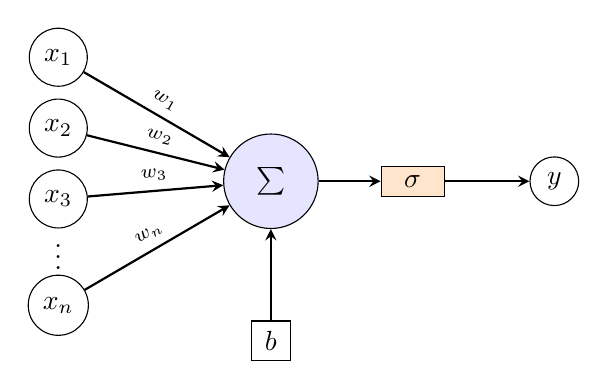
\begin{tikzpicture}[>=stealth, scale=0.9]
        % Inputs
        \node[circle, draw, minimum size=0.6cm] (x1) at (0, 2) {$x_{1}$};
        \node[circle, draw, minimum size=0.6cm] (x2) at (0, 1) {$x_{2}$};
        \node[circle, draw, minimum size=0.6cm] (x3) at (0, 0) {$x_{3}$};
        \node at (0, -0.7) {$\vdots$};
        \node[circle, draw, minimum size=0.6cm] (xn) at (0, -1.5) {$x_{n}$};

        % Neuron
        \node[circle, draw, minimum size=1.2cm, fill=blue!10] (neuron) at (3, 0.25) {$\sum$};
        \node[rectangle, draw, minimum width=0.8cm, fill=orange!20] (sigma) at (5, 0.25) {$\sigma$};

        % Output
        \node[circle, draw, minimum size=0.6cm] (y) at (7, 0.25) {$y$};

        % Bias
        \node[rectangle, draw, minimum size=0.5cm] (b) at (3, -2) {$b$};

        % Connections
        \draw[->, thick] (x1) -- (neuron) node[midway, above, sloped, font=\scriptsize] {$w_1$};
        \draw[->, thick] (x2) -- (neuron) node[midway, above, sloped, font=\scriptsize] {$w_2$};
        \draw[->, thick] (x3) -- (neuron) node[midway, above, sloped, font=\scriptsize] {$w_3$};
        \draw[->, thick] (xn) -- (neuron) node[midway, above, sloped, font=\scriptsize] {$w_n$};
        \draw[->, thick] (b) -- (neuron);
        \draw[->, thick] (neuron) -- (sigma);
        \draw[->, thick] (sigma) -- (y);
    \end{tikzpicture}
\caption{A single neuron: weighted sum of inputs plus bias, followed by activation function.}
\end{figure}

\begin{remark}[Geometric Interpretation]
    The pre-activation $z = \mathbf{w}^\top \mathbf{x} + b$ defines a hyperplane in $\mathbb{R}^n$:
    \begin{itemize}
        \item The hyperplane $\{\mathbf{x} : \mathbf{w}^\top \mathbf{x} + b = 0\}$ divides the input space
        \item $\mathbf{w}$ is the normal vector to this hyperplane
        \item $b$ controls the offset from the origin
        \item The activation $\sigma$ introduces nonlinearity, allowing the network to learn non-linear decision boundaries
    \end{itemize}
\end{remark}

\begin{remark}[Layer of Neurons]
    A \textbf{layer} consists of $m$ neurons operating in parallel on the same input:
    \[
        \mathbf{y} = \sigma(W\mathbf{x} + \mathbf{b})
    \]
    where $W \in \mathbb{R}^{m \times n}$ stacks the weight vectors as rows, $\mathbf{b} \in \mathbb{R}^m$ contains all biases, and $\sigma$ is applied element-wise.
\end{remark}

\begin{figure}[h]
\centering
    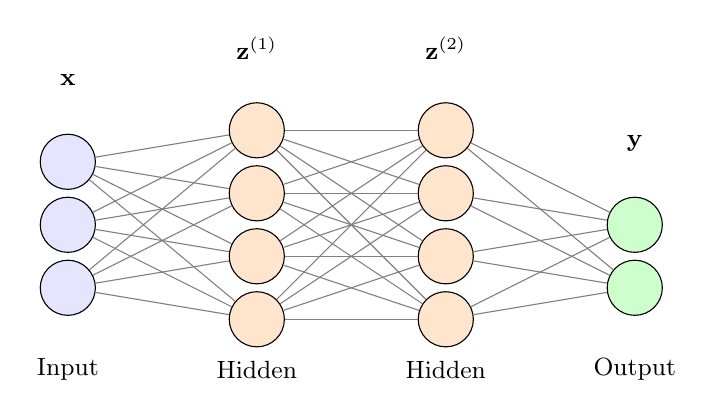
\begin{tikzpicture}[>=stealth, scale=0.8]
        % Input layer
        \foreach \i in {1,2,3} {
            \node[circle, draw, minimum size=0.7cm, fill=blue!10] (i\i) at (0, 2-\i) {};
        }
        \node at (0, -2.3) {\small Input};

        % Hidden layer 1
        \foreach \i in {1,2,3,4} {
            \node[circle, draw, minimum size=0.7cm, fill=orange!20] (h1\i) at (3, 2.5-\i) {};
        }
        \node at (3, -2.3) {\small Hidden};

        % Hidden layer 2
        \foreach \i in {1,2,3,4} {
            \node[circle, draw, minimum size=0.7cm, fill=orange!20] (h2\i) at (6, 2.5-\i) {};
        }
        \node at (6, -2.3) {\small Hidden};

        % Output layer
        \foreach \i in {1,2} {
            \node[circle, draw, minimum size=0.7cm, fill=green!20] (o\i) at (9, 1-\i) {};
        }
        \node at (9, -2.3) {\small Output};

        % Connections input to hidden1
        \foreach \i in {1,2,3} {
            \foreach \j in {1,2,3,4} {
                \draw[-, gray, thin] (i\i) -- (h1\j);
            }
        }

        % Connections hidden1 to hidden2
        \foreach \i in {1,2,3,4} {
            \foreach \j in {1,2,3,4} {
                \draw[-, gray, thin] (h1\i) -- (h2\j);
            }
        }

        % Connections hidden2 to output
        \foreach \i in {1,2,3,4} {
            \foreach \j in {1,2} {
                \draw[-, gray, thin] (h2\i) -- (o\j);
            }
        }

        % Layer labels
        \node at (0, 2.3) {\small $\mathbf{x}$};
        \node at (3, 2.8) {\small $\mathbf{z}^{(1)}$};
        \node at (6, 2.8) {\small $\mathbf{z}^{(2)}$};
        \node at (9, 1.3) {\small $\mathbf{y}$};
    \end{tikzpicture}
\caption{Feedforward neural network with two hidden layers. Each layer applies a linear transformation followed by a nonlinear activation.}
\end{figure}

% ============================================================
\section{Activation Functions}

Without nonlinear activation functions, a neural network collapses to a single linear transformation regardless of depth. Activation functions introduce the nonlinearity that makes deep learning powerful.

\begin{definition}[Sigmoid]
    The \textbf{sigmoid} (or logistic) function squashes inputs to $(0, 1)$:
    \[
        \sigma(x) = \frac{1}{1 + e^{-x}}
    \]
    Properties: $\sigma(0) = 0.5$, $\sigma'(x) = \sigma(x)(1 - \sigma(x))$, and $\lim_{x \to \pm\infty} \sigma(x) = \{1, 0\}$.
\end{definition}

\begin{definition}[Hyperbolic Tangent]
    The \textbf{tanh} function squashes inputs to $(-1, 1)$:
    \[
        \tanh(x) = \frac{e^x - e^{-x}}{e^x + e^{-x}} = 2\sigma(2x) - 1
    \]
    Zero-centered unlike sigmoid, which often improves optimization.
\end{definition}

\begin{definition}[ReLU]
    The \textbf{Rectified Linear Unit} is the most widely used activation:
    \[
        \text{ReLU}(x) = \max(0, x) = \begin{cases} x & x > 0 \\ 0 & x \leq 0 \end{cases}
    \]
    Computationally efficient and avoids vanishing gradients for $x > 0$. However, neurons can ``die'' if they always receive negative inputs (gradient becomes zero).
\end{definition}

\begin{figure}[h]
\centering
    \begin{tikzpicture}[scale=0.75, baseline=(current bounding box.south)]
        % Sigmoid
        \begin{scope}
            \draw[->] (-3,0) -- (3,0) node[right] {$x$};
            \draw[->] (0,-1.5) -- (0,1.5);
            \draw[thick, blue, domain=-3:3, samples=50] plot (\x, {1/(1+exp(-\x))});
            \draw[dashed, gray] (-3,1) -- (3,1);
            \node at (0,-2) {\small Sigmoid};
        \end{scope}

        % Tanh
        \begin{scope}[shift={(7,0)}]
            \draw[->] (-3,0) -- (3,0) node[right] {$x$};
            \draw[->] (0,-1.5) -- (0,1.5);
            \draw[thick, red, domain=-3:3, samples=50] plot (\x, {tanh(\x)});
            \draw[dashed, gray] (-3,1) -- (3,1);
            \draw[dashed, gray] (-3,-1) -- (3,-1);
            \node at (0,-2) {\small Tanh};
        \end{scope}

        % ReLU
        \begin{scope}[shift={(14,0)}]
            \draw[->] (-3,0) -- (3,0) node[right] {$x$};
            \draw[->] (0,-1.5) -- (0,2.5);
            \draw[thick, green!70!black, domain=-3:0] plot (\x, 0);
            \draw[thick, green!70!black, domain=0:2.3] plot (\x, \x);
            \node at (0,-2) {\small ReLU};
        \end{scope}
    \end{tikzpicture}
\caption{Common activation functions. Sigmoid saturates at 0 and 1; tanh is zero-centered; ReLU is piecewise linear.}
\end{figure}

% ============================================================
\section{Loss Functions}

To train a neural network, we need to quantify how well it performs. A \emph{loss function} measures the discrepancy between predictions and targets.

\begin{definition}[Loss Function]
    A \textbf{loss function} $\mathcal{L}: \mathcal{Y} \times \mathcal{Y} \to \mathbb{R}_{\geq 0}$ measures the error between a prediction $\hat{y}$ and target $y$. For a dataset $\{(\mathbf{x}_i, y_i)\}_{i=1}^{N}$, the \textbf{empirical risk} is:
    \[
        \mathcal{L}(\theta) = \frac{1}{N} \sum_{i=1}^{N} \ell(f_\theta(\mathbf{x}_i), y_i)
    \]
    where $f_\theta$ is the neural network with parameters $\theta$ and $\ell$ is the per-sample loss.
\end{definition}

\begin{definition}[Mean Squared Error]
    For regression tasks, the \textbf{mean squared error (MSE)} loss is:
    \[
        \ell_{\text{MSE}}(\hat{y}, y) = \frac{1}{2}(\hat{y} - y)^2
    \]
    For vector outputs:
    \[
        \ell_{\text{MSE}}(\hat{\mathbf{y}}, \mathbf{y}) = \frac{1}{2}\|\hat{\mathbf{y}} - \mathbf{y}\|_2^2 = \frac{1}{2}\sum_{j} (\hat{y}_j - y_j)^2
    \]
\end{definition}

\begin{definition}[Cross-Entropy Loss]
    For classification with $K$ classes, let $(p_1, \ldots, p_K)$ be the predicted probabilities (output of softmax, so $p_k \geq 0$ and $\sum_k p_k = 1$) and $y \in \{1, \ldots, K\}$ be the true class. The \textbf{cross-entropy loss} is:
    \[
        \ell_{\text{CE}}(p, y) = -\log p_y
    \]
    Using one-hot encoding $\mathbf{y} = \mathbf{e}_y$ (the $y$-th standard basis vector):
    \[
        \ell_{\text{CE}}(p, \mathbf{y}) = -\sum_{k=1}^{K} y_k \log p_k
    \]
\end{definition}

\begin{remark}[Cross-Entropy and KL Divergence]
    Cross-entropy relates to KL divergence (see \cref{def:kl-divergence}) via:
    \[
        H(q, p) = D_{\mathrm{KL}}(q \| p) + H(q)
    \]
    where $q$ is the true distribution and $p$ is the predicted. For one-hot $q$ (a single true class), $H(q) = 0$, so minimizing cross-entropy is equivalent to minimizing KL divergence.
\end{remark}

\begin{definition}[Softmax]
    The \textbf{softmax} function converts logits $\mathbf{z} \in \mathbb{R}^K$ to a probability distribution:
    \[
        \text{softmax}(\mathbf{z})_k = \frac{e^{z_k}}{\sum_{j=1}^{K} e^{z_j}} = \frac{\exp(z_k)}{\|\exp(\mathbf{z})\|_1}
    \]
    This is the gradient of the log-sum-exp function: $\nabla_\mathbf{z} \log\sum_k e^{z_k} = \text{softmax}(\mathbf{z})$.
\end{definition}

\begin{proposition}[Softmax-Cross-Entropy Gradient]
    Let $\mathbf{z}$ be logits, $p = \text{softmax}(\mathbf{z})$, and $y$ be the true class. The gradient of the cross-entropy loss with respect to logits is:
    \[
        \frac{\partial \ell_{\text{CE}}}{\partial z_k} = p_k - \mathbf{1}_{[k=y]}
    \]
    Or in vector form: $\nabla_\mathbf{z} \ell_{\text{CE}} = p - \mathbf{e}_y$.
\end{proposition}

\begin{proof}
    Write $\ell = -\log p_y = -z_y + \log\sum_{j} e^{z_j}$. Then:
    \[
        \frac{\partial \ell}{\partial z_k} = -\mathbf{1}_{[k=y]} + \frac{e^{z_k}}{\sum_j e^{z_j}} = -\mathbf{1}_{[k=y]} + p_k = p_k - \mathbf{1}_{[k=y]}
    \]
\end{proof}

\begin{definition}[Binary Cross-Entropy]
    For binary classification with prediction $p \in [0,1]$ (output of sigmoid) and label $y \in \{0,1\}$:
    \[
        \ell_{\text{BCE}}(p, y) = -y\log p - (1-y)\log(1-p)
    \]
    This is equivalent to cross-entropy for $K=2$ classes.
\end{definition}

\begin{figure}[h]
\centering
    \begin{tikzpicture}[scale=0.9]
        % MSE loss
        \begin{scope}
            \draw[->] (-2.5,0) -- (2.5,0) node[right] {$\hat{y} - y$};
            \draw[->] (0,-0.3) -- (0,3) node[above] {$\ell$};
            \draw[thick, blue, domain=-1.7:1.7, samples=50] plot (\x, {0.5*\x*\x});
            \node at (0,-0.7) {\small MSE: $\frac{1}{2}(\hat{y}-y)^2$};
        \end{scope}

        % Cross-entropy loss (y=1)
        \begin{scope}[shift={(7,0)}]
            \draw[->] (0,0) -- (3.5,0) node[right] {$p$};
            \draw[->] (0,-0.3) -- (0,3) node[above] {$\ell$};
            \draw[thick, red, domain=0.05:3, samples=50] plot (\x, {-ln(\x/3)});
            \node[below] at (3, 0) {\small $1$};
            \node[below] at (0, 0) {\small $0$};
            \node at (1.5,-0.7) {\small CE ($y{=}1$): $-\log p$};
        \end{scope}
    \end{tikzpicture}
\caption{Loss function shapes: MSE penalizes errors quadratically; cross-entropy penalizes confident wrong predictions heavily.}
\end{figure}

% ============================================================
\section{Gradient Descent}

Training a neural network amounts to finding parameters $\theta$ that minimize the loss $\mathcal{L}(\theta)$. Gradient descent iteratively moves in the direction of steepest descent.

\begin{definition}[Gradient Descent]
    \textbf{Gradient descent} updates parameters by:
    \[
        \theta_{t+1} = \theta_t - \eta \nabla_\theta \mathcal{L}(\theta_t)
    \]
    where $\eta > 0$ is the \textbf{learning rate} (step size).
\end{definition}

\begin{figure}[h]
\centering
    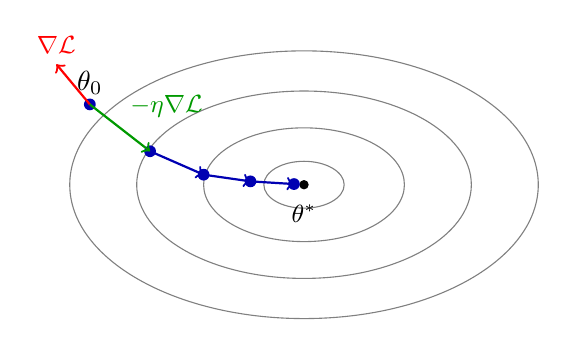
\begin{tikzpicture}[scale=0.85]
        % Loss surface contours
        \draw[gray] (0,0) ellipse (3.5cm and 2cm);
        \draw[gray] (0,0) ellipse (2.5cm and 1.4cm);
        \draw[gray] (0,0) ellipse (1.5cm and 0.85cm);
        \draw[gray] (0,0) ellipse (0.6cm and 0.35cm);
        \fill (0,0) circle (2pt);
        \node[below] at (0,-0.15) {\small $\theta^*$};

        % Gradient descent path
        \coordinate (p0) at (-3.2, 1.2);
        \coordinate (p1) at (-2.3, 0.5);
        \coordinate (p2) at (-1.5, 0.15);
        \coordinate (p3) at (-0.8, 0.05);
        \coordinate (p4) at (-0.15, 0.01);

        \foreach \i in {0,1,2,3,4} {
            \fill[blue!70!black] (p\i) circle (2.5pt);
        }
        \draw[->, thick, blue!70!black] (p1) -- (p2);
        \draw[->, thick, blue!70!black] (p2) -- (p3);
        \draw[->, thick, blue!70!black] (p3) -- (p4);

        \node[above] at (p0) {$\theta_0$};

        % Gradient vectors at theta_0
        \draw[->, thick, red] (p0) -- ++(-0.5, 0.6) node[above] {\small $\nabla\mathcal{L}$};
        \draw[->, thick, green!60!black] (p0) -- (p1) node[midway, above right] {\small $-\eta\nabla\mathcal{L}$};
    \end{tikzpicture}
\caption{Gradient descent on a loss surface. Contours represent level sets; the path moves toward the minimum $\theta^*$.}
\end{figure}

\begin{remark}[Motivation from Taylor Expansion]
    Gradient descent emerges naturally from asking: \emph{given our current position $\theta$, which direction should we move to decrease $\mathcal{L}$?}

    The \textbf{first-order Taylor expansion} approximates the loss near $\theta$:
    \[
        \mathcal{L}(\theta + \Delta\theta) \approx \mathcal{L}(\theta) + \nabla \mathcal{L}(\theta)^\top \Delta\theta
    \]
    This is a linear approximation---we're replacing the curved loss surface with its tangent hyperplane. To decrease $\mathcal{L}$, we need $\nabla \mathcal{L}^\top \Delta\theta < 0$.

    \textbf{Which direction minimizes this?} For a fixed step size $\|\Delta\theta\| = \epsilon$, by Cauchy-Schwarz:
    \[
        \nabla \mathcal{L}^\top \Delta\theta \geq -\|\nabla\mathcal{L}\| \cdot \|\Delta\theta\| = -\epsilon\|\nabla\mathcal{L}\|
    \]
    with equality when $\Delta\theta = -\epsilon \cdot \nabla\mathcal{L}/\|\nabla\mathcal{L}\|$. Thus the \textbf{negative gradient is the direction of steepest descent}.
\end{remark}

\begin{remark}[Comparison with Newton-Raphson]
    The Newton-Raphson method finds \textbf{roots} of a function $g(\theta) = 0$:
    \[
        \theta_{t+1} = \theta_t - \frac{g(\theta_t)}{g'(\theta_t)}
    \]

    For optimization, we don't want $\mathcal{L}(\theta) = 0$ (that would just find where the loss is zero). Instead, we want \textbf{critical points} where $\nabla\mathcal{L}(\theta) = 0$---the minima.

    So we apply Newton-Raphson to $g = \nabla\mathcal{L}$. The derivative of the gradient is the Hessian: $g' = \nabla^2\mathcal{L}$. This gives \textbf{Newton's method}:
    \[
        \theta_{t+1} = \theta_t - [\nabla^2 \mathcal{L}(\theta_t)]^{-1} \nabla\mathcal{L}(\theta_t)
    \]

    \textbf{Key difference}: Gradient descent uses only first-order information (the gradient), while Newton's method uses second-order information (the Hessian). Gradient descent follows the slope; Newton's method accounts for how the slope itself is changing.
\end{remark}

\begin{definition}[Stochastic Gradient Descent (SGD)]
    Computing the full gradient requires a forward and backward pass through all $N$ samples. With $N$ in the millions and each pass taking $O(P)$ operations (where $P$ is the number of parameters), one gradient step costs $O(NP)$---too slow for practical training. \textbf{Stochastic gradient descent} uses a random \textbf{minibatch} $\mathcal{B} \subset \{1, \ldots, N\}$:
    \[
        \theta_{t+1} = \theta_t - \eta \cdot \frac{1}{|\mathcal{B}|} \sum_{i \in \mathcal{B}} \nabla_\theta \ell(f_\theta(\mathbf{x}_i), y_i)
    \]
    The minibatch gradient is an unbiased estimate. If we sample $|\mathcal{B}|$ indices i.i.d.\ uniformly from $\{1,\ldots,N\}$:
    \[
        \mathbb{E}\left[\frac{1}{|\mathcal{B}|} \sum_{k=1}^{|\mathcal{B}|} \nabla \ell_{i_k}\right] = \frac{1}{|\mathcal{B}|} \sum_{k=1}^{|\mathcal{B}|} \underbrace{\mathbb{E}[\nabla\ell_{i_k}]}_{= \frac{1}{N}\sum_{j=1}^{N}\nabla\ell_j} = \frac{1}{N}\sum_{j=1}^{N} \nabla \ell_j = \nabla \mathcal{L}
    \]
\end{definition}

\begin{remark}[Batch Size Trade-offs]\leavevmode
    \begin{itemize}
        \item \textbf{Small batches}: High variance in gradient estimates, but more updates per epoch. Noise acts as regularization.
        \item \textbf{Large batches}: Lower variance, more accurate gradients, better hardware utilization. May converge to sharp minima and generalize worse.
        \item \textbf{Examples}: ResNet-50 on ImageNet used batch size 256. GPT-3 175B used 3.2M tokens per batch. DeepSeek-V3 ramped batch size from 3,072 to 15,360 during training.
    \end{itemize}
\end{remark}

% ============================================================
\section{Second-Order Methods and the Hessian}

First-order methods like gradient descent use only $\nabla\mathcal{L}$. Second-order methods additionally use the \textbf{Hessian matrix} to capture curvature information.

\begin{definition}[Second-Order Taylor Expansion]
    The second-order Taylor expansion of $\mathcal{L}$ around $\theta$ is:
    \[
        \mathcal{L}(\theta + \Delta\theta) \approx \mathcal{L}(\theta) + \nabla\mathcal{L}(\theta)^\top \Delta\theta + \frac{1}{2}\Delta\theta^\top \mathbf{H}(\theta) \Delta\theta
    \]
    where $\mathbf{H}(\theta) = \nabla^2\mathcal{L}(\theta)$ is the \textbf{Hessian matrix} with entries:
    \[
        H_{ij} = \frac{\partial^2 \mathcal{L}}{\partial \theta_i \partial \theta_j}
    \]
    The Hessian is symmetric (assuming continuous second derivatives) and captures how the gradient changes as we move in parameter space.
\end{definition}

\begin{remark}[Geometric Interpretation of the Hessian]
    The Hessian encodes the \textbf{curvature} of the loss surface:
    \begin{itemize}
        \item \textbf{Eigenvalues}: The eigenvalues $\lambda_i$ of $\mathbf{H}$ give the curvature along each eigenvector direction. Large $\lambda_i$ means steep curvature (loss changes rapidly); small $\lambda_i$ means flat curvature.
        \item \textbf{Condition number}: $\kappa = \lambda_{\max}/\lambda_{\min}$ measures how ``stretched'' the loss surface is. High $\kappa$ means elongated contours---gradient descent zigzags and converges slowly.
        \item \textbf{Positive definiteness}: If $\mathbf{H} \succ 0$ (all eigenvalues positive), the point is a local minimum. If $\mathbf{H}$ has negative eigenvalues, it's a saddle point or maximum.
    \end{itemize}
\end{remark}

\begin{definition}[Newton's Method]
    To find the optimal step, we minimize the quadratic approximation:
    \[
        \min_{\Delta\theta} \left[ \nabla\mathcal{L}^\top \Delta\theta + \frac{1}{2}\Delta\theta^\top \mathbf{H} \Delta\theta \right]
    \]
    Taking the gradient and setting to zero: $\nabla\mathcal{L} + \mathbf{H}\Delta\theta = 0$, giving:
    \[
        \Delta\theta^* = -\mathbf{H}^{-1}\nabla\mathcal{L}
    \]
    This yields \textbf{Newton's method}:
    \[
        \theta_{t+1} = \theta_t - \mathbf{H}(\theta_t)^{-1} \nabla\mathcal{L}(\theta_t)
    \]
\end{definition}

\begin{remark}[Why Newton's Method is Better (When It Works)]
    Newton's method has compelling advantages:
    \begin{itemize}
        \item \textbf{Quadratic convergence}: Near a minimum, the error decreases as $\|\theta_{t+1} - \theta^*\| \leq C\|\theta_t - \theta^*\|^2$. Gradient descent only achieves linear convergence.
        \item \textbf{Affine invariance}: Newton's method is invariant to linear reparameterizations. If we change coordinates $\phi = A\theta$, Newton's path is unchanged. Gradient descent's path depends on the parameterization.
        \item \textbf{Automatic step size}: The Hessian naturally scales the step---large steps in flat directions, small steps in steep directions.
    \end{itemize}
\end{remark}

\begin{remark}[Why We Don't Use Newton's Method in Deep Learning]
    Despite its theoretical appeal, pure Newton's method is impractical for neural networks:
    \begin{itemize}
        \item \textbf{Storage}: For $P$ parameters, $\mathbf{H}$ is $P \times P$. GPT-3 has $P = 175\text{B}$; storing $\mathbf{H}$ would require $175\text{B}^2 \cdot 4$ bytes $\approx 10^{23}$ bytes---more than all storage on Earth.
        \item \textbf{Computation}: Computing $\mathbf{H}$ requires $O(P^2)$ second derivatives. Inverting it costs $O(P^3)$.
        \item \textbf{Non-convexity}: Neural network losses are non-convex. $\mathbf{H}$ may be indefinite, making $\mathbf{H}^{-1}\nabla\mathcal{L}$ point toward saddle points rather than minima.
    \end{itemize}
\end{remark}

\begin{remark}[Practical Approximations]\leavevmode
    \begin{itemize}
        \item \textbf{Diagonal approximation}: Use only $\text{diag}(\mathbf{H})$, giving per-parameter learning rates. This is the idea behind AdaGrad/Adam.
        \item \textbf{Quasi-Newton (BFGS, L-BFGS)}: Build an approximate $\mathbf{H}^{-1}$ from gradient differences. L-BFGS stores only $O(mP)$ values for $m \approx 10$. Works well for small networks but struggles with stochastic gradients.
        \item \textbf{Gauss-Newton}: For least-squares losses, approximate $\mathbf{H} \approx \mathbf{J}^\top\mathbf{J}$ where $\mathbf{J}$ is the Jacobian. Always positive semi-definite.
        \item \textbf{Natural gradient}: Use the Fisher information matrix $\mathbf{F}$ instead of $\mathbf{H}$. This measures curvature in \emph{distribution space} rather than parameter space.
        \item \textbf{K-FAC}: Approximate $\mathbf{F}$ as a Kronecker product of smaller matrices, reducing cost to $O(P)$.
    \end{itemize}
\end{remark}

\begin{figure}[h]
\centering
    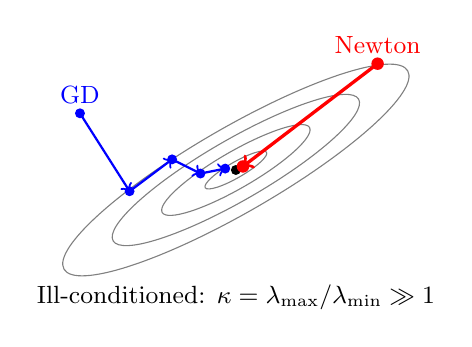
\begin{tikzpicture}[scale=0.9]
        % Elongated contours
        \begin{scope}
            \draw[gray, rotate=30] (0,0) ellipse (2.8cm and 0.6cm);
            \draw[gray, rotate=30] (0,0) ellipse (2.0cm and 0.43cm);
            \draw[gray, rotate=30] (0,0) ellipse (1.2cm and 0.26cm);
            \draw[gray, rotate=30] (0,0) ellipse (0.5cm and 0.11cm);
            \fill (0,0) circle (2pt);

            % Gradient descent path (zigzag)
            \coordinate (g0) at (-2.2, 0.8);
            \coordinate (g1) at (-1.5, -0.3);
            \coordinate (g2) at (-0.9, 0.15);
            \coordinate (g3) at (-0.5, -0.05);
            \coordinate (g4) at (-0.15, 0.02);

            \draw[->, thick, blue] (g0) -- (g1);
            \draw[->, thick, blue] (g1) -- (g2);
            \draw[->, thick, blue] (g2) -- (g3);
            \draw[->, thick, blue] (g3) -- (g4);
            \foreach \i in {0,1,2,3,4} {
                \fill[blue] (g\i) circle (2pt);
            }
            \node[above, blue] at (g0) {\small GD};

            % Newton path (direct)
            \coordinate (n0) at (2.0, 1.5);
            \draw[->, thick, red, line width=1.2pt] (n0) -- (0.1, 0.05);
            \fill[red] (n0) circle (2.5pt);
            \fill[red] (0.1, 0.05) circle (2.5pt);
            \node[above, red] at (n0) {\small Newton};

            \node at (0, -1.8) {\small Ill-conditioned: $\kappa = \lambda_{\max}/\lambda_{\min} \gg 1$};
        \end{scope}
    \end{tikzpicture}
\caption{Gradient descent zigzags on ill-conditioned problems (high condition number), while Newton's method goes directly to the minimum by accounting for curvature.}
\end{figure}

% ============================================================
\section{Backpropagation}

Backpropagation efficiently computes gradients by applying the chain rule layer-by-layer, reusing intermediate computations.

\begin{theorem}[Backpropagation]
    Consider a neural network as a composition $f = f_L \circ f_{L-1} \circ \cdots \circ f_1$ with loss $\mathcal{L} = \ell \circ f$. Let $\mathbf{z}^{(\ell)}$ denote the output of layer $\ell$ (with $\mathbf{z}^{(0)} = \mathbf{x}$). The gradient with respect to parameters in layer $\ell$ is:
    \[
        \frac{\partial \mathcal{L}}{\partial \theta_\ell} = \frac{\partial \mathcal{L}}{\partial \mathbf{z}^{(\ell)}} \cdot \frac{\partial \mathbf{z}^{(\ell)}}{\partial \theta_\ell}
    \]
    where the ``upstream gradient'' $\partial \mathcal{L}/\partial \mathbf{z}^{(\ell)}$ is computed recursively:
    \[
        \frac{\partial \mathcal{L}}{\partial \mathbf{z}^{(\ell-1)}} = \frac{\partial \mathcal{L}}{\partial \mathbf{z}^{(\ell)}} \cdot \frac{\partial \mathbf{z}^{(\ell)}}{\partial \mathbf{z}^{(\ell-1)}}
    \]
\end{theorem}

\begin{remark}[Forward and Backward Passes]
    Backpropagation consists of two phases:
    \begin{enumerate}
        \item \textbf{Forward pass}: Compute all activations $\mathbf{z}^{(1)}, \ldots, \mathbf{z}^{(L)}$ and the loss $\mathcal{L}$.
        \item \textbf{Backward pass}: Starting from $\partial\mathcal{L}/\partial\mathbf{z}^{(L)}$, propagate gradients backward through each layer.
    \end{enumerate}
    Each intermediate activation must be stored during the forward pass for use in the backward pass. This is the primary memory cost of training.
\end{remark}

\begin{figure}[h]
\centering
    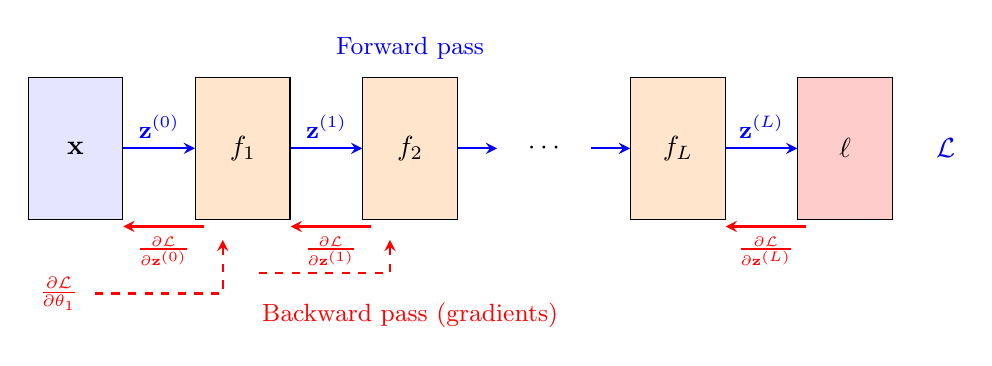
\begin{tikzpicture}[>=stealth, scale=0.85]
        % Layers
        \node[draw, rectangle, minimum width=1.2cm, minimum height=1.8cm, fill=blue!10] (x) at (0,0) {$\mathbf{x}$};
        \node[draw, rectangle, minimum width=1.2cm, minimum height=1.8cm, fill=orange!20] (l1) at (2.5,0) {$f_1$};
        \node[draw, rectangle, minimum width=1.2cm, minimum height=1.8cm, fill=orange!20] (l2) at (5,0) {$f_2$};
        \node at (7,0) {$\cdots$};
        \node[draw, rectangle, minimum width=1.2cm, minimum height=1.8cm, fill=orange!20] (lL) at (9,0) {$f_L$};
        \node[draw, rectangle, minimum width=1.2cm, minimum height=1.8cm, fill=red!20] (loss) at (11.5,0) {$\ell$};

        % Forward arrows (top)
        \draw[->, thick, blue] (x.east) -- (l1.west) node[midway, above] {\small $\mathbf{z}^{(0)}$};
        \draw[->, thick, blue] (l1.east) -- (l2.west) node[midway, above] {\small $\mathbf{z}^{(1)}$};
        \draw[->, thick, blue] (l2.east) -- (6.3,0);
        \draw[->, thick, blue] (7.7,0) -- (lL.west);
        \draw[->, thick, blue] (lL.east) -- (loss.west) node[midway, above] {\small $\mathbf{z}^{(L)}$};
        \node[blue] at (13, 0) {$\mathcal{L}$};

        % Backward arrows (bottom)
        \draw[<-, thick, red, dashed] (l1.south) ++(-0.3,-0.3) -- ++(0,-0.8) -- ++(-2,0) node[left] {\small $\frac{\partial \mathcal{L}}{\partial \theta_1}$};
        \draw[<-, thick, red, dashed] (l2.south) ++(-0.3,-0.3) -- ++(0,-0.5) -- ++(-2,0);

        % Gradient flow
        \draw[<-, thick, red] (x.south east) ++(0,-0.1) -- ++(1.2,0) node[midway, below] {\scriptsize $\frac{\partial \mathcal{L}}{\partial \mathbf{z}^{(0)}}$};
        \draw[<-, thick, red] (l1.south east) ++(0,-0.1) -- ++(1.2,0) node[midway, below] {\scriptsize $\frac{\partial \mathcal{L}}{\partial \mathbf{z}^{(1)}}$};
        \draw[<-, thick, red] (lL.south east) ++(0,-0.1) -- ++(1.2,0) node[midway, below] {\scriptsize $\frac{\partial \mathcal{L}}{\partial \mathbf{z}^{(L)}}$};

        % Labels
        \node[blue] at (5, 1.5) {\small Forward pass};
        \node[red] at (5, -2.5) {\small Backward pass (gradients)};
    \end{tikzpicture}
\caption{Backpropagation: forward pass computes activations; backward pass propagates gradients via the chain rule.}
\end{figure}

\begin{example}[Backprop Through a Linear Layer]
    Consider layer $\mathbf{z} = W\mathbf{a} + \mathbf{b}$ where $\mathbf{a}$ is the input (previous layer's activation). Given upstream gradient $\boldsymbol{\delta} = \partial\mathcal{L}/\partial\mathbf{z}$:
    \begin{align}
        \frac{\partial \mathcal{L}}{\partial W} &= \boldsymbol{\delta} \mathbf{a}^\top & &\text{(outer product)} \\[4pt]
        \frac{\partial \mathcal{L}}{\partial \mathbf{b}} &= \boldsymbol{\delta} & &\text{(direct)} \\[4pt]
        \frac{\partial \mathcal{L}}{\partial \mathbf{a}} &= W^\top \boldsymbol{\delta} & &\text{(propagate to previous layer)}
    \end{align}
\end{example}

\begin{example}[Backprop Through Activations]
    For element-wise activation $\mathbf{a} = \sigma(\mathbf{z})$, given upstream gradient $\boldsymbol{\delta} = \partial\mathcal{L}/\partial\mathbf{a}$:
    \[
        \frac{\partial \mathcal{L}}{\partial \mathbf{z}} = \boldsymbol{\delta} \odot \sigma'(\mathbf{z})
    \]
    where $\odot$ denotes element-wise multiplication. For ReLU: $\sigma'(z) = \mathbf{1}_{[z > 0]}$, so gradients are ``gated'' by whether the neuron was active.
\end{example}

\begin{remark}[Jacobian Perspective]
    For a function $\mathbf{f}: \mathbb{R}^n \to \mathbb{R}^m$, the Jacobian $J_\mathbf{f} \in \mathbb{R}^{m \times n}$ has entries $(J_\mathbf{f})_{ij} = \partial f_i/\partial x_j$. The chain rule becomes matrix multiplication:
    \[
        J_{\mathbf{g} \circ \mathbf{f}} = J_\mathbf{g} \cdot J_\mathbf{f}
    \]
    Backpropagation computes the \emph{vector-Jacobian product} (VJP) $\mathbf{v}^\top J$ efficiently without forming the full Jacobian. This is why we propagate row vectors (gradients) backward, not column vectors.
\end{remark}

\begin{proposition}[Computational Complexity]
    Let the forward pass require $F$ floating-point operations. The backward pass requires approximately $2F$ operations---roughly twice the forward pass. This is because each operation in the forward pass corresponds to one multiplication and one addition in the backward pass.
\end{proposition}

% ============================================================
\section{Optimization Algorithms}

Plain SGD can be slow and sensitive to the learning rate. Modern optimizers adapt the learning rate and use momentum to accelerate convergence.

\begin{definition}[Momentum]
    \textbf{SGD with momentum} maintains a velocity term that accumulates past gradients:
    \begin{align}
        \mathbf{v}_{t+1} &= \beta \mathbf{v}_t + \nabla \mathcal{L}(\theta_t) \\
        \theta_{t+1} &= \theta_t - \eta \mathbf{v}_{t+1}
    \end{align}
    where $\beta \in [0,1)$ is the momentum coefficient (typically $\beta = 0.9$).
\end{definition}

\begin{remark}[Why Momentum Works]
    Momentum provides two benefits:
    \begin{itemize}
        \item \textbf{Acceleration}: In consistent gradient directions, velocity builds up, allowing faster progress.
        \item \textbf{Noise reduction}: Random fluctuations average out while consistent directions reinforce.
    \end{itemize}

    Viewing the sequence as an exponential moving average: if gradients are constant $\mathbf{g}$, then $\mathbf{v} \to \mathbf{g}/(1-\beta)$, amplifying the effective step size.
\end{remark}

\begin{figure}[h]
\centering
    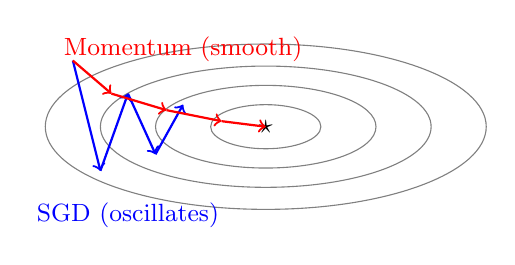
\begin{tikzpicture}[scale=0.7]
        % Loss surface contours
        \draw[gray, thin] (0,0) ellipse (4cm and 1.5cm);
        \draw[gray, thin] (0,0) ellipse (3cm and 1.1cm);
        \draw[gray, thin] (0,0) ellipse (2cm and 0.75cm);
        \draw[gray, thin] (0,0) ellipse (1cm and 0.4cm);
        \node at (0,0) {$\star$};

        % SGD path (oscillating)
        \draw[blue, thick, ->] (-3.5, 1.2) -- (-3, -0.8);
        \draw[blue, thick, ->] (-3, -0.8) -- (-2.5, 0.6);
        \draw[blue, thick, ->] (-2.5, 0.6) -- (-2, -0.5);
        \draw[blue, thick, ->] (-2, -0.5) -- (-1.5, 0.4);
        \node[blue, below] at (-2.5, -1.2) {\small SGD (oscillates)};

        % Momentum path (smooth)
        \draw[red, thick, ->] (-3.5, 1.2) -- (-2.8, 0.6);
        \draw[red, thick, ->] (-2.8, 0.6) -- (-1.8, 0.3);
        \draw[red, thick, ->] (-1.8, 0.3) -- (-0.8, 0.1);
        \draw[red, thick, ->] (-0.8, 0.1) -- (0, 0);
        \node[red, above] at (-1.5, 1) {\small Momentum (smooth)};
    \end{tikzpicture}
\caption{SGD oscillates in directions with high curvature; momentum smooths the trajectory by accumulating velocity.}
\end{figure}

\begin{definition}[AdaGrad]
    \textbf{AdaGrad} adapts the learning rate for each parameter based on historical gradients:
    \begin{align}
        \mathbf{s}_{t+1} &= \mathbf{s}_t + (\nabla \mathcal{L}(\theta_t))^2 & &\text{(accumulate squared gradients)} \\
        \theta_{t+1} &= \theta_t - \frac{\eta}{\sqrt{\mathbf{s}_{t+1}} + \epsilon} \odot \nabla \mathcal{L}(\theta_t)
    \end{align}
    where operations are element-wise and $\epsilon \approx 10^{-8}$ prevents division by zero.
\end{definition}

\begin{remark}[AdaGrad Intuition]
    Parameters with large gradients get smaller learning rates; those with small gradients get larger rates. This is useful for sparse features: rare features get larger updates when they do appear. The downside: learning rates only decrease, which can cause premature stopping.
\end{remark}

\begin{definition}[RMSProp]
    \textbf{RMSProp} fixes AdaGrad's diminishing learning rate by using an exponential moving average:
    \begin{align}
        \mathbf{s}_{t+1} &= \rho\, \mathbf{s}_t + (1-\rho)(\nabla \mathcal{L}(\theta_t))^2 \\
        \theta_{t+1} &= \theta_t - \frac{\eta}{\sqrt{\mathbf{s}_{t+1}} + \epsilon} \odot \nabla \mathcal{L}(\theta_t)
    \end{align}
    where $\rho \approx 0.9$ controls the decay rate.
\end{definition}

\begin{definition}[Adam]
    \textbf{Adam} (Adaptive Moment Estimation) combines momentum with adaptive learning rates:
    \begin{align}
        \mathbf{m}_{t+1} &= \beta_1 \mathbf{m}_t + (1-\beta_1) \nabla \mathcal{L}(\theta_t) & &\text{(first moment)} \\
        \mathbf{v}_{t+1} &= \beta_2 \mathbf{v}_t + (1-\beta_2) (\nabla \mathcal{L}(\theta_t))^2 & &\text{(second moment)} \\
        \hat{\mathbf{m}}_{t+1} &= \frac{\mathbf{m}_{t+1}}{1 - \beta_1^{t+1}} & &\text{(bias correction)} \\
        \hat{\mathbf{v}}_{t+1} &= \frac{\mathbf{v}_{t+1}}{1 - \beta_2^{t+1}} & &\text{(bias correction)} \\
        \theta_{t+1} &= \theta_t - \frac{\eta}{\sqrt{\hat{\mathbf{v}}_{t+1}} + \epsilon} \odot \hat{\mathbf{m}}_{t+1}
    \end{align}
    Default hyperparameters: $\beta_1 = 0.9$, $\beta_2 = 0.999$, $\epsilon = 10^{-8}$.
\end{definition}

\begin{remark}[Bias Correction]
    The bias correction terms $1/(1-\beta^t)$ compensate for the initialization $\mathbf{m}_0 = \mathbf{v}_0 = \mathbf{0}$. Without correction, early estimates are biased toward zero. As $t \to \infty$, the correction approaches 1.
\end{remark}

\begin{definition}[AdamW]
    \textbf{AdamW} decouples weight decay from the adaptive learning rate:
    \[
        \theta_{t+1} = \theta_t - \eta\left(\frac{\hat{\mathbf{m}}_{t+1}}{\sqrt{\hat{\mathbf{v}}_{t+1}} + \epsilon} + \lambda \theta_t\right)
    \]
    where $\lambda$ is the weight decay coefficient. In standard Adam with L2 regularization, the weight decay is scaled by the adaptive learning rate, which is undesirable.
\end{definition}

\begin{remark}[Practical Recommendations]
    \begin{itemize}
        \item \textbf{AdamW} is the default choice for transformers and most deep learning.
        \item \textbf{SGD with momentum} can generalize better but requires more tuning; often used for CNNs.
        \item Learning rate schedules (warmup, cosine decay) are essential for good performance.
        \item The learning rate is typically the most important hyperparameter to tune.
    \end{itemize}
\end{remark}

% ============================================================
\section{Universal Approximation}

Neural networks are powerful because they can approximate any continuous function to arbitrary precision.

\begin{theorem}[Universal Approximation---Cybenko, 1989]
    Let $\sigma: \mathbb{R} \to \mathbb{R}$ be a continuous sigmoidal function (i.e., $\sigma(x) \to 1$ as $x \to \infty$ and $\sigma(x) \to 0$ as $x \to -\infty$). Then for any continuous function $f: [0,1]^n \to \mathbb{R}$ and any $\epsilon > 0$, there exists a single-hidden-layer network:
    \[
        g(\mathbf{x}) = \sum_{j=1}^{m} \alpha_j \sigma(\mathbf{w}_j^\top \mathbf{x} + b_j)
    \]
    such that $\sup_{\mathbf{x} \in [0,1]^n} |f(\mathbf{x}) - g(\mathbf{x})| < \epsilon$.
\end{theorem}

\begin{remark}[What This Means]
    \begin{itemize}
        \item A single hidden layer with enough neurons can approximate any continuous function.
        \item This is an \textbf{existence} result---it doesn't say how many neurons are needed (could be exponentially many) or how to find the weights.
        \item Modern extensions show ReLU networks are also universal approximators.
    \end{itemize}
\end{remark}

\begin{remark}[Width vs Depth]
    Universal approximation holds for width (wide shallow networks), but:
    \begin{itemize}
        \item \textbf{Wide networks}: Can approximate any function, but may need exponentially many neurons.
        \item \textbf{Deep networks}: Can represent certain functions exponentially more efficiently. Some functions require exponential width with bounded depth but polynomial size with sufficient depth.
    \end{itemize}

    In practice, deep networks generalize better and are more parameter-efficient. The residual stream interpretation (next section) explains why depth helps: each layer can incrementally refine the representation.
\end{remark}

\begin{theorem}[Depth Separation]
    There exist functions computable by depth-$k$ networks of polynomial size that require exponential size for depth-$(k-1)$ networks. That is, depth provably helps for some function classes.
\end{theorem}

% ============================================================
\section{Residual Connections and the Residual Stream}

\begin{definition}[Residual Connection]
    A \textbf{residual connection} (or skip connection) adds the input of a layer to its output:
    \[
        y = x + F(x)
    \]
    where $F$ is the layer's learned transformation. Instead of learning $y = F(x)$ directly, the network learns the \emph{residual} $F(x) = y - x$.
\end{definition}

\begin{remark}[Why Residuals Work]
    The key insight is that learning $F(x) \approx 0$ (doing nothing) is easy---just set weights to zero. This provides:
    \begin{itemize}
        \item \textbf{Easy identity}: If a layer isn't needed, it can learn to pass input through unchanged
        \item \textbf{Gradient flow}: Gradients flow directly through the addition, avoiding vanishing gradients
        \item \textbf{Depth without degradation}: Deeper networks can't perform worse than shallower ones
    \end{itemize}
\end{remark}

\begin{definition}[Residual Stream]
    The \textbf{residual stream} is a conceptual framework for understanding transformers. Think of a ``river'' of information flowing through the network:
    \[
        x^{(0)} \xrightarrow{+\text{Attn}_1} x^{(1)} \xrightarrow{+\text{MLP}_1} x^{(2)} \xrightarrow{+\text{Attn}_2} \cdots \xrightarrow{+\text{MLP}_L} x^{(2L)}
    \]
    Each component \emph{reads from} and \emph{writes to} this shared stream via addition.
\end{definition}

\begin{figure}[h]
\centering
    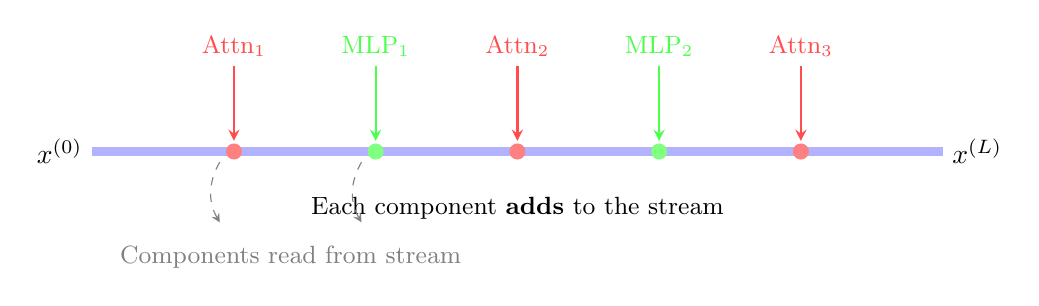
\begin{tikzpicture}[>=stealth, scale=0.9]
        % Main stream
        \draw[line width=3pt, blue!30] (0,0) -- (12,0);
        \node[left] at (0,0) {$x^{(0)}$};
        \node[right] at (12,0) {$x^{(L)}$};

        % Components writing to stream
        \foreach \x/\label/\col in {2/Attn$_1$/red, 4/MLP$_1$/green, 6/Attn$_2$/red, 8/MLP$_2$/green, 10/Attn$_3$/red} {
            \draw[->, thick, \col!70] (\x, 1.2) -- (\x, 0.15);
            \node[above, \col!70] at (\x, 1.2) {\small \label};
            \filldraw[\col!50] (\x, 0) circle (3pt);
        }

        % Labels
        \node[below] at (6, -0.5) {\small Each component \textbf{adds} to the stream};

        % Reading arrows
        \draw[->, dashed, gray] (1.8, -0.15) to[bend right=30] (1.8, -1);
        \draw[->, dashed, gray] (3.8, -0.15) to[bend right=30] (3.8, -1);
        \node[below, gray] at (2.8, -1.2) {\small Components read from stream};
    \end{tikzpicture}
\caption{The residual stream: attention and MLP layers read from and write to a shared representation via addition.}
\end{figure}

\begin{remark}[Residual Stream Interpretation]
    This view reveals important properties:
    \begin{itemize}
        \item \textbf{Superposition}: The stream holds a superposition of features from all previous layers
        \item \textbf{Direct paths}: Information from layer 1 can directly influence layer 10 via the residual
        \item \textbf{Additive contributions}: Each layer's contribution can be analyzed independently
        \item \textbf{No information destruction}: Layers add information; they don't overwrite it
    \end{itemize}

    Mathematically, the final output is:
    \[
        x^{(L)} = x^{(0)} + \sum_{\ell=1}^{L} F_\ell(x^{(\ell-1)})
    \]
    The output is the input plus the sum of all layer contributions.
\end{remark}

% ============================================================
\section{The FFN Block}

In transformers, the \textbf{FFN block} (feedforward block) is a specific two-layer network applied independently at each token position.

\begin{definition}[FFN Block]
    The \textbf{FFN block} in a transformer is:
    \[
        \text{FFN}(x) = W_2 \, \sigma(W_1 x + b_1) + b_2
    \]
    where:
    \begin{itemize}
        \item $x \in \mathbb{R}^{d_{\text{model}}}$ is the input (one token's representation)
        \item $W_1 \in \mathbb{R}^{d_{\text{ff}} \times d_{\text{model}}}$ projects to a higher dimension
        \item $\sigma$ is a nonlinear activation (GELU, SiLU, etc.)
        \item $W_2 \in \mathbb{R}^{d_{\text{model}} \times d_{\text{ff}}}$ projects back down
        \item Typically $d_{\text{ff}} = 4 \cdot d_{\text{model}}$
    \end{itemize}
\end{definition}

\begin{figure}[h]
\centering
    \begin{tikzpicture}[>=stealth, node distance=1.5cm]
        % Input
        \node[draw, minimum width=1cm, minimum height=2cm, fill=blue!10] (in) {$x$};
        \node[below=0.1cm of in] {\small $d_{\text{model}}$};

        % W1
        \node[draw, minimum width=1.5cm, minimum height=3cm, fill=orange!20, right=1cm of in] (w1) {$W_1$};

        % Hidden
        \node[draw, minimum width=1cm, minimum height=3cm, fill=green!10, right=1cm of w1] (h) {$\sigma(\cdot)$};
        \node[below=0.1cm of h] {\small $d_{\text{ff}} = 4d$};

        % W2
        \node[draw, minimum width=1.5cm, minimum height=2cm, fill=orange!20, right=1cm of h] (w2) {$W_2$};

        % Output
        \node[draw, minimum width=1cm, minimum height=2cm, fill=blue!10, right=1cm of w2] (out) {$y$};
        \node[below=0.1cm of out] {\small $d_{\text{model}}$};

        % Arrows
        \draw[->, thick] (in) -- (w1);
        \draw[->, thick] (w1) -- (h);
        \draw[->, thick] (h) -- (w2);
        \draw[->, thick] (w2) -- (out);

        % Labels
        \node[above=0.3cm of w1] {\small expand};
        \node[above=0.3cm of w2] {\small compress};
    \end{tikzpicture}
\caption{FFN block: expand to higher dimension, apply nonlinearity, then compress back to model dimension.}
\end{figure}

\begin{remark}[FFN as Key-Value Memory]
    The FFN can be interpreted as an associative memory:
    \begin{itemize}
        \item Rows of $W_1$ are \textbf{keys} (patterns to detect)
        \item Columns of $W_2$ are \textbf{values} (information to retrieve)
        \item $\sigma(W_1 x)$ computes ``match scores'' for each key
        \item $W_2 \sigma(W_1 x)$ retrieves a weighted combination of values
    \end{itemize}

    This is where factual knowledge (``Paris is the capital of France'') appears to be stored. The keys detect contexts like ``The capital of France is'', and values provide the completion.
\end{remark}

\begin{remark}[Position Independence]
    Critically, the FFN is applied \textbf{independently to each position}:
    \[
        \text{FFN}([x_1, x_2, \ldots, x_n]) = [\text{FFN}(x_1), \text{FFN}(x_2), \ldots, \text{FFN}(x_n)]
    \]
    There is no communication between positions in the FFN---that's the job of attention. The FFN processes each token's representation in isolation.
\end{remark}

% ============================================================
\section{Modern Activation Functions}

Beyond ReLU, modern architectures (especially transformers) use smoother activations:

\begin{definition}[GELU]
    The \textbf{Gaussian Error Linear Unit}:
    \[
        \text{GELU}(x) = x \cdot \Phi(x) \approx x \cdot \frac{1}{2}\left[1 + \tanh\left(\sqrt{\frac{2}{\pi}}(x + 0.044715 x^3)\right)\right]
    \]
    where $\Phi$ is the standard normal CDF. Smooth approximation to ReLU; used in GPT, BERT.
\end{definition}

\begin{definition}[SiLU/Swish]
    The \textbf{Sigmoid Linear Unit} (also called Swish):
    \[
        \text{SiLU}(x) = x \cdot \sigma(x) = \frac{x}{1 + e^{-x}}
    \]
    Smooth, non-monotonic, self-gated. Used in many modern architectures.
\end{definition}

\begin{definition}[SwiGLU]
    The \textbf{Swish-Gated Linear Unit} combines SiLU with gating:
    \[
        \text{SwiGLU}(x) = \text{SiLU}(W_1 x) \odot (W_3 x)
    \]
    Uses an extra projection $W_3$ for gating. Used in LLaMA, PaLM.
\end{definition}

\begin{figure}[h]
\centering
    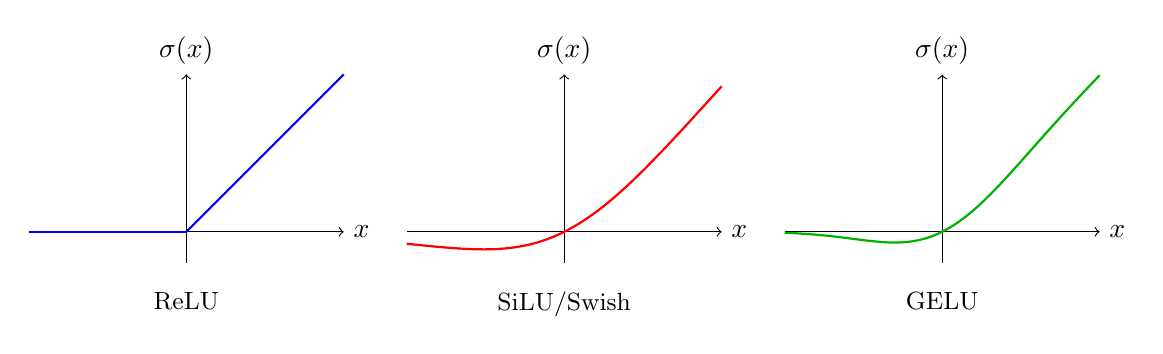
\begin{tikzpicture}[scale=0.8]
        \begin{scope}
            \draw[->] (-2.5,0) -- (2.5,0) node[right] {$x$};
            \draw[->] (0,-0.5) -- (0,2.5) node[above] {$\sigma(x)$};
            \draw[thick, blue, domain=-2.5:0] plot (\x, 0);
            \draw[thick, blue, domain=0:2.5] plot (\x, \x);
            \node[below] at (0,-0.8) {\small ReLU};
        \end{scope}

        \begin{scope}[shift={(6,0)}]
            \draw[->] (-2.5,0) -- (2.5,0) node[right] {$x$};
            \draw[->] (0,-0.5) -- (0,2.5) node[above] {$\sigma(x)$};
            \draw[thick, red, domain=-2.5:2.5, samples=50] plot (\x, {\x/(1+exp(-\x))});
            \node[below] at (0,-0.8) {\small SiLU/Swish};
        \end{scope}

        \begin{scope}[shift={(12,0)}]
            \draw[->] (-2.5,0) -- (2.5,0) node[right] {$x$};
            \draw[->] (0,-0.5) -- (0,2.5) node[above] {$\sigma(x)$};
            \draw[thick, green!70!black, domain=-2.5:2.5, samples=50] plot (\x, {0.5*\x*(1+tanh(0.7978*(\x + 0.044715*\x*\x*\x)))});
            \node[below] at (0,-0.8) {\small GELU};
        \end{scope}
    \end{tikzpicture}
\caption{Modern activation functions: ReLU is piecewise linear; SiLU and GELU are smooth approximations used in transformers.}
\end{figure}

% ============================================================
\section{General Feedforward Neural Networks (MLP)}

Having seen the specific FFN block used in transformers, we now define the general concept.

\begin{definition}[Feedforward Neural Network / MLP]
    A \textbf{feedforward neural network} (or \textbf{multilayer perceptron}) is a composition of layers:
    \[
        f(x) = (f_L \circ f_{L-1} \circ \cdots \circ f_1)(x)
    \]
    where each layer $f_\ell(z) = \sigma(W_\ell z + b_\ell)$ applies a linear transformation followed by a nonlinearity.

    Equivalently:
    \[
        f(x) = W_L \sigma(W_{L-1} \sigma(\cdots \sigma(W_1 x + b_1) \cdots) + b_{L-1}) + b_L
    \]
\end{definition}

\begin{remark}[Terminology]
    \textbf{``Feedforward''} means information flows in one direction (input $\to$ output) with no cycles. This contrasts with recurrent networks where outputs feed back as inputs.

    \textbf{``Multilayer perceptron''} is historical---the original perceptron used step functions; modern MLPs use smooth activations. The name persists.

    The transformer's FFN block is a specific 2-layer MLP with expansion ratio 4.
\end{remark}

% ============================================================
\section{Embeddings}

\begin{definition}[Embedding]
    An \textbf{embedding} is a learned mapping from discrete objects to continuous vectors:
    \[
        \text{Embed}: \mathcal{V} \to \mathbb{R}^d
    \]
    where $\mathcal{V}$ is a finite vocabulary and $d$ is the embedding dimension.
\end{definition}

\begin{remark}[Implementation]
    Embeddings are stored as a matrix $E \in \mathbb{R}^{|\mathcal{V}| \times d}$ where row $i$ is the embedding of token $i$. Lookup is just indexing: $\text{Embed}(t) = E[i, :]$.

    Equivalently, this is multiplication by a one-hot vector:
    \[
        \text{Embed}(t) = \mathbf{1}_t^\top E
    \]
\end{remark}

\begin{remark}[Why Embeddings?]
    \textbf{Problem}: Discrete tokens have no inherent similarity. Token indices are arbitrary.

    \textbf{Solution}: Learn a continuous space where:
    \begin{itemize}
        \item Similar items have similar vectors
        \item Relationships are encoded as directions (``king $-$ man $+$ woman $\approx$ queen'')
        \item The geometry captures meaningful structure
    \end{itemize}
\end{remark}

% ============================================================
\chapter{Transformer Theory}

\section{Self-Attention Mechanism}

\begin{definition}[Scaled Dot-Product Attention]
    Given queries $Q$, keys $K$, and values $V$:
    \[
        \text{Attention}(Q, K, V) = \text{softmax}\left(\frac{QK^\top}{\sqrt{d_k}}\right) V
    \]
    The attention weights $A = \text{softmax}(QK^\top / \sqrt{d_k})$ form a stochastic matrix where $A_{ij}$ is how much position $i$ attends to position $j$.
\end{definition}

\begin{definition}[Self-Attention]
    In \textbf{self-attention}, queries, keys, and values all come from the same sequence:
    \[
        Q = XW_Q, \quad K = XW_K, \quad V = XW_V
    \]
    where $X \in \mathbb{R}^{n \times d}$ is the input sequence and $W_Q, W_K, W_V$ are learned projections.
\end{definition}

\begin{remark}[Dimension Analysis]
    Let us trace the dimensions carefully:
    \begin{itemize}
        \item Input: $X \in \mathbb{R}^{n \times d_{\text{model}}}$ (sequence of $n$ tokens, each $d_{\text{model}}$-dimensional)
        \item Projections: $W_Q, W_K \in \mathbb{R}^{d_{\text{model}} \times d_k}$ and $W_V \in \mathbb{R}^{d_{\text{model}} \times d_v}$
        \item Queries/Keys: $Q, K \in \mathbb{R}^{n \times d_k}$
        \item Values: $V \in \mathbb{R}^{n \times d_v}$
        \item Attention scores: $QK^\top \in \mathbb{R}^{n \times n}$
        \item Attention weights: $A = \text{softmax}(QK^\top/\sqrt{d_k}) \in \mathbb{R}^{n \times n}$
        \item \textbf{Output}: $AV \in \mathbb{R}^{n \times d_v}$
    \end{itemize}

    \textbf{Key observation}: The output dimension equals $d_v$ (the value dimension), not $d_k$ (the key/query dimension). The attention matrix $A$ is $n \times n$; multiplying by $V$ (which is $n \times d_v$) gives $n \times d_v$.

    In practice, typically $d_k = d_v = d_{\text{model}} / H$ where $H$ is the number of heads.
\end{remark}

\begin{figure}[h]
\centering
    \begin{tikzpicture}[>=stealth, scale=0.7]
        % Step 1: Q × K^T = A
        \node[above, font=\small\bfseries] at (3, 1.8) {Step 1: Compute attention scores};

        % Q
        \node[draw, minimum width=1.2cm, minimum height=2cm, fill=blue!15] (Q) at (0, 0) {$Q$};
        \node[below=0.1cm of Q, font=\small] {$n \times d_k$};

        % K^T
        \node[draw, minimum width=2cm, minimum height=1.2cm, fill=red!15] (K) at (2.5, 0) {$K^\top$};
        \node[below=0.1cm of K, font=\small] {$d_k \times n$};

        % = A
        \node at (4.3, 0) {$=$};
        \node[draw, minimum width=2cm, minimum height=2cm, fill=purple!15] (A) at (6, 0) {$A$};
        \node[below=0.1cm of A, font=\small] {$n \times n$};
    \end{tikzpicture}
    \hspace{1cm}
    \begin{tikzpicture}[>=stealth, scale=0.7]
        % Step 2: A × V = Out
        \node[above, font=\small\bfseries] at (3, 1.8) {Step 2: Weighted sum of values};

        % A
        \node[draw, minimum width=2cm, minimum height=2cm, fill=purple!15] (A) at (0, 0) {$A$};
        \node[below=0.1cm of A, font=\small] {$n \times n$};

        % V
        \node[draw, minimum width=1.5cm, minimum height=2cm, fill=green!15] (V) at (3, 0) {$V$};
        \node[below=0.1cm of V, font=\small] {$n \times d_v$};

        % = output
        \node at (4.8, 0) {$=$};
        \node[draw, minimum width=1.5cm, minimum height=2cm, fill=orange!15] (O) at (6.5, 0) {Out};
        \node[below=0.1cm of O, font=\small] {$n \times d_v$};
    \end{tikzpicture}
\caption{Attention as matrix multiplication: (1) query-key products yield attention weights; (2) weights aggregate values.}
\end{figure}

% ============================================================
\section{Multi-Head Attention}

Single-head attention can only learn one type of relationship pattern. Multi-head attention runs multiple attention operations in parallel, allowing the model to simultaneously attend to information from different representation subspaces.

\begin{definition}[Multi-Head Attention]
    Given $H$ attention heads, \textbf{multi-head attention} computes:
    \[
        \text{MultiHead}(Q, K, V) = \text{Concat}(\text{head}_1, \ldots, \text{head}_H) W_O
    \]
    where each head uses its own projections:
    \[
        \text{head}_h = \text{Attention}(XW_Q^{(h)}, XW_K^{(h)}, XW_V^{(h)})
    \]
    with $W_Q^{(h)}, W_K^{(h)} \in \mathbb{R}^{d_{\text{model}} \times d_k}$, $W_V^{(h)} \in \mathbb{R}^{d_{\text{model}} \times d_v}$, and the output projection $W_O \in \mathbb{R}^{Hd_v \times d_{\text{model}}}$.
\end{definition}

\begin{remark}[Intuition: Why Multiple Heads?]
    Consider the sentence: ``\textit{The cat sat on the mat because it was tired.}''

    Different relationships exist simultaneously:
    \begin{itemize}
        \item \textbf{Syntactic}: ``it'' $\to$ ``cat'' (pronoun resolution)
        \item \textbf{Positional}: ``sat'' $\to$ ``on'' (adjacent dependency)
        \item \textbf{Semantic}: ``tired'' $\to$ ``cat'' (who is tired?)
        \item \textbf{Causal}: ``sat'' $\to$ ``tired'' (why did it sit?)
    \end{itemize}

    A single attention pattern cannot capture all these simultaneously. Each head can specialize in one type of pattern.
\end{remark}

\begin{figure}[h]
\centering
    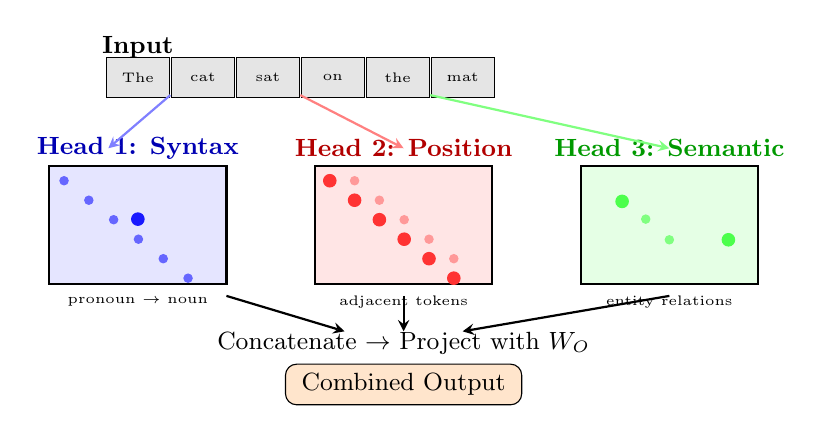
\begin{tikzpicture}[>=stealth, scale=0.75]
        % Input sequence
        \node[font=\small\bfseries] at (0, 4.5) {Input};
        \foreach \i/\word in {0/The, 1/cat, 2/sat, 3/on, 4/the, 5/mat} {
            \node[draw, minimum width=0.8cm, minimum height=0.5cm, fill=gray!20] at (\i*1.1, 4) {\tiny \word};
        }

        % Head 1: Syntactic
        \begin{scope}[shift={(-1.5, 0)}]
            \node[font=\small\bfseries, blue!70!black] at (1.5, 2.8) {Head 1: Syntax};
            \draw[thick, fill=blue!10] (0, 0.5) rectangle (3, 2.5);
            % Attention pattern: strong diagonal + some structure
            \foreach \i in {0,...,5} {
                \filldraw[blue!60] (0.25 + \i*0.42, 2.25 - \i*0.33) circle (2pt);
            }
            % "it" -> "cat" pattern
            \filldraw[blue!90] (1.5, 1.6) circle (3pt);
            \node[font=\tiny] at (1.5, 0.2) {pronoun $\to$ noun};
        \end{scope}

        % Head 2: Positional
        \begin{scope}[shift={(3, 0)}]
            \node[font=\small\bfseries, red!70!black] at (1.5, 2.8) {Head 2: Position};
            \draw[thick, fill=red!10] (0, 0.5) rectangle (3, 2.5);
            % Strong diagonal pattern
            \foreach \i in {0,...,5} {
                \filldraw[red!80] (0.25 + \i*0.42, 2.25 - \i*0.33) circle (3pt);
            }
            % Adjacent attention
            \foreach \i in {0,...,4} {
                \filldraw[red!40] (0.67 + \i*0.42, 2.25 - \i*0.33) circle (2pt);
            }
            \node[font=\tiny] at (1.5, 0.2) {adjacent tokens};
        \end{scope}

        % Head 3: Semantic
        \begin{scope}[shift={(7.5, 0)}]
            \node[font=\small\bfseries, green!60!black] at (1.5, 2.8) {Head 3: Semantic};
            \draw[thick, fill=green!10] (0, 0.5) rectangle (3, 2.5);
            % More distributed pattern
            \filldraw[green!70] (0.7, 1.9) circle (3pt);  % cat
            \filldraw[green!70] (2.5, 1.25) circle (3pt); % mat
            \filldraw[green!50] (1.1, 1.6) circle (2pt);  % sat
            \filldraw[green!50] (1.5, 1.25) circle (2pt);
            \node[font=\tiny] at (1.5, 0.2) {entity relations};
        \end{scope}

        % Arrows from input to heads
        \draw[->, thick, blue!50] (0.55, 3.7) -- (-0.5, 2.8);
        \draw[->, thick, red!50] (2.75, 3.7) -- (4.5, 2.8);
        \draw[->, thick, green!50] (4.95, 3.7) -- (9, 2.8);

        % Concatenation
        \node at (4.5, -0.5) {\small Concatenate $\to$ Project with $W_O$};
        \draw[->, thick] (1.5, 0.3) -- (3.5, -0.3);
        \draw[->, thick] (4.5, 0.3) -- (4.5, -0.3);
        \draw[->, thick] (9, 0.3) -- (5.5, -0.3);

        % Output
        \node[draw, rounded corners, fill=orange!20, minimum width=3cm] at (4.5, -1.2) {\small Combined Output};
    \end{tikzpicture}
\caption{Multi-head attention: each head learns a different attention pattern, then outputs are concatenated and projected.}
\end{figure}

\begin{example}[Observed Head Specialization]
    Research analyzing trained transformers has found heads that specialize in:

    \begin{itemize}
        \item \textbf{Previous token heads}: Attend strongly to position $i-1$
        \item \textbf{Induction heads}: Attend to tokens that followed similar contexts (covered later)
        \item \textbf{Rare word heads}: Focus attention on uncommon tokens
        \item \textbf{Delimiter heads}: Attend to punctuation and separators
        \item \textbf{Duplicate token heads}: Find repeated tokens in the sequence
        \item \textbf{Syntax heads}: Track grammatical structure (subject-verb, noun-adjective)
    \end{itemize}

    Not all heads are equally important---some can be pruned with minimal performance loss.
\end{example}

\begin{remark}[Dimension Budget]
    To keep computation constant, the per-head dimension is reduced:
    \[
        d_k = d_v = \frac{d_{\text{model}}}{H}
    \]

    For GPT-3 with $d_{\text{model}} = 12288$ and $H = 96$ heads: $d_k = 128$ per head.

    This means each head operates in a lower-dimensional subspace, forcing each head to focus on specific patterns rather than learning everything.
\end{remark}

\begin{figure}[h]
\centering
    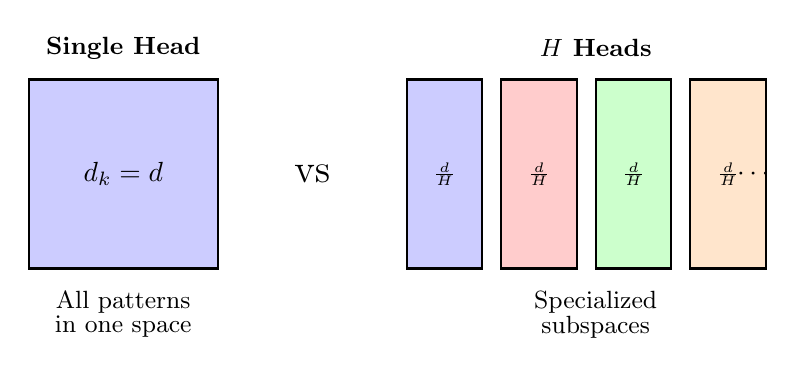
\begin{tikzpicture}[>=stealth, scale=0.8]
        % Single head (large)
        \begin{scope}
            \node[font=\small\bfseries] at (1.5, 3.5) {Single Head};
            \draw[thick, fill=blue!20] (0, 0) rectangle (3, 3);
            \node at (1.5, 1.5) {$d_k = d$};
            \node[below, font=\small] at (1.5, -0.2) {All patterns};
            \node[below, font=\small] at (1.5, -0.6) {in one space};
        \end{scope}

        \node at (4.5, 1.5) {\Large vs};

        % Multiple heads (smaller)
        \begin{scope}[shift={(6, 0)}]
            \node[font=\small\bfseries] at (3, 3.5) {$H$ Heads};
            \foreach \i/\col in {0/blue, 1/red, 2/green, 3/orange} {
                \draw[thick, fill=\col!20] (\i*1.5, 0) rectangle (\i*1.5 + 1.2, 3);
                \node at (\i*1.5 + 0.6, 1.5) {\tiny $\frac{d}{H}$};
            }
            \node at (5.5, 1.5) {$\cdots$};
            \node[below, font=\small] at (3, -0.2) {Specialized};
            \node[below, font=\small] at (3, -0.6) {subspaces};
        \end{scope}
    \end{tikzpicture}
\caption{Single head uses full dimension; multiple heads partition into specialized subspaces.}
\end{figure}

\begin{remark}[Why Concatenate Then Project?]
    After computing all heads, we concatenate and apply $W_O$:
    \[
        \text{Output} = [\text{head}_1; \ldots; \text{head}_H] W_O
    \]

    The output projection $W_O$ serves several purposes:
    \begin{itemize}
        \item \textbf{Mixing}: Combines information from different heads
        \item \textbf{Dimension matching}: Maps $Hd_v$ back to $d_{\text{model}}$
        \item \textbf{Learning}: Allows the model to learn how to weight different heads' contributions
    \end{itemize}

    Without $W_O$, heads would be independent and couldn't share information.
\end{remark}

% ============================================================
\section{Why Divide by $\sqrt{d_k}$?}

The scaling factor $\sqrt{d_k}$ in attention is not arbitrary---it is precisely the factor needed to control the variance of dot products and prevent softmax saturation.

\begin{theorem}[Variance of Dot Products]
    Let $q, k \in \mathbb{R}^{d_k}$ be random vectors with independent components satisfying $\mathbb{E}[q_i] = \mathbb{E}[k_i] = 0$ and $\text{Var}(q_i) = \text{Var}(k_i) = 1$. Then:
    \[
        \mathbb{E}[q^\top k] = 0 \quad \text{and} \quad \text{Var}(q^\top k) = d_k
    \]
\end{theorem}

\begin{proof}
    The dot product is $q^\top k = \sum_{i=1}^{d_k} q_i k_i$. We compute its mean and variance.

    \textbf{Mean}:
    \[
        \mathbb{E}[q^\top k] = \mathbb{E}\left[\sum_{i=1}^{d_k} q_i k_i\right] = \sum_{i=1}^{d_k} \mathbb{E}[q_i k_i] = \sum_{i=1}^{d_k} \mathbb{E}[q_i] \mathbb{E}[k_i] = \sum_{i=1}^{d_k} 0 \cdot 0 = 0
    \]
    where we used independence of $q_i$ and $k_i$.

    \textbf{Variance}: Since $\mathbb{E}[q^\top k] = 0$, we have $\text{Var}(q^\top k) = \mathbb{E}[(q^\top k)^2]$.
    \begin{align*}
        \mathbb{E}[(q^\top k)^2] &= \mathbb{E}\left[\left(\sum_{i=1}^{d_k} q_i k_i\right)^2\right] \\
        &= \mathbb{E}\left[\sum_{i=1}^{d_k} \sum_{j=1}^{d_k} q_i k_i q_j k_j\right] \\
        &= \sum_{i=1}^{d_k} \sum_{j=1}^{d_k} \mathbb{E}[q_i k_i q_j k_j]
    \end{align*}

    For $i \neq j$, by independence:
    \[
        \mathbb{E}[q_i k_i q_j k_j] = \mathbb{E}[q_i]\mathbb{E}[k_i]\mathbb{E}[q_j]\mathbb{E}[k_j] = 0
    \]

    For $i = j$:
    \[
        \mathbb{E}[q_i^2 k_i^2] = \mathbb{E}[q_i^2] \mathbb{E}[k_i^2] = \text{Var}(q_i) \cdot \text{Var}(k_i) = 1 \cdot 1 = 1
    \]

    Therefore:
    \[
        \text{Var}(q^\top k) = \sum_{i=1}^{d_k} 1 = d_k
    \]
\end{proof}

\begin{corollary}[Standard Deviation Scaling]
    The standard deviation of the dot product is $\sqrt{d_k}$. To obtain unit variance:
    \[
        \text{Var}\left(\frac{q^\top k}{\sqrt{d_k}}\right) = \frac{\text{Var}(q^\top k)}{d_k} = \frac{d_k}{d_k} = 1
    \]
    This is why we divide by $\sqrt{d_k}$, not $d_k$.
\end{corollary}

\begin{remark}[Why Variance Control Matters for Softmax]
    The softmax function is:
    \[
        \text{softmax}(z)_i = \frac{e^{z_i}}{\sum_j e^{z_j}}
    \]

    When inputs $z_i$ have large magnitude, softmax \textbf{saturates}:

    \begin{center}
        \begin{tabular}{l|l|l}
            \textbf{Input} & \textbf{Output} & \textbf{Gradient} \\
            \hline
            $[1, 0, 0, 0]$ & $[0.46, 0.18, 0.18, 0.18]$ & Healthy \\
            $[5, 0, 0, 0]$ & $[0.95, 0.02, 0.02, 0.02]$ & Reduced \\
            $[10, 0, 0, 0]$ & $[0.9999, 10^{-4}, 10^{-4}, 10^{-4}]$ & Nearly zero \\
        \end{tabular}
    \end{center}

    \textbf{Problem}: With $d_k = 64$, unscaled dot products have standard deviation $\sqrt{64} = 8$. Values of $\pm 16$ (two standard deviations) are common, causing extreme saturation.

    \textbf{Solution}: Dividing by $\sqrt{d_k} = 8$ brings the standard deviation back to 1, keeping softmax in a well-behaved regime.
\end{remark}

\begin{figure}[h]
\centering
    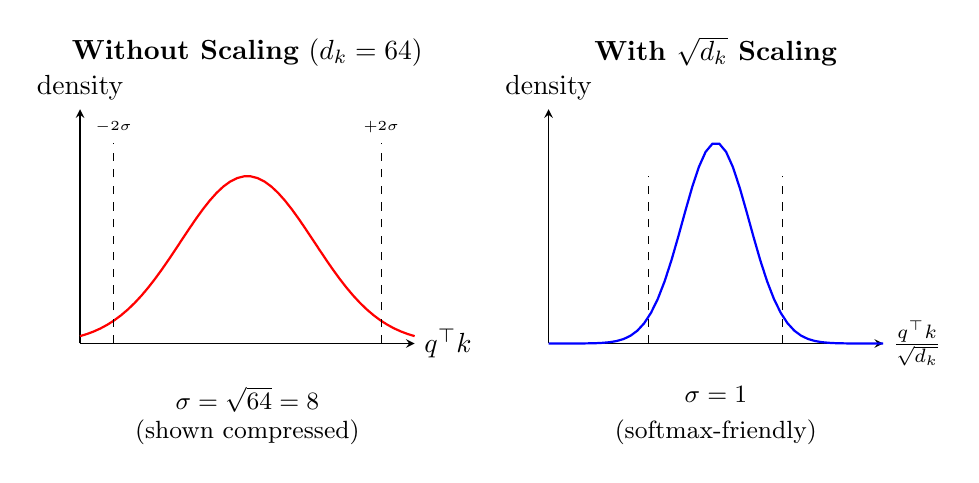
\begin{tikzpicture}[>=stealth, scale=0.85]
        % Without scaling
        \begin{scope}
            \node[above] at (2.5, 4) {\textbf{Without Scaling} ($d_k = 64$)};
            \draw[->] (0,0) -- (5,0) node[right] {$q^\top k$};
            \draw[->] (0,0) -- (0,3.5) node[above] {density};

            % Wide distribution
            \draw[thick, red, domain=0:5, samples=50] plot (\x, {2.5*exp(-(\x-2.5)^2/2)});
            \draw[dashed] (0.5, 0) -- (0.5, 3) node[above, font=\tiny] {$-2\sigma$};
            \draw[dashed] (4.5, 0) -- (4.5, 3) node[above, font=\tiny] {$+2\sigma$};

            \node[below] at (2.5, -0.5) {\small $\sigma = \sqrt{64} = 8$};
            \node[below] at (2.5, -1) {\small (shown compressed)};
        \end{scope}

        % With scaling
        \begin{scope}[shift={(7,0)}]
            \node[above] at (2.5, 4) {\textbf{With $\sqrt{d_k}$ Scaling}};
            \draw[->] (0,0) -- (5,0) node[right] {$\frac{q^\top k}{\sqrt{d_k}}$};
            \draw[->] (0,0) -- (0,3.5) node[above] {density};

            % Narrow distribution
            \draw[thick, blue, domain=0:5, samples=50] plot (\x, {3*exp(-(\x-2.5)^2/0.5)});
            \draw[dashed] (1.5, 0) -- (1.5, 2.5);
            \draw[dashed] (3.5, 0) -- (3.5, 2.5);

            \node[below] at (2.5, -0.5) {\small $\sigma = 1$};
            \node[below] at (2.5, -1) {\small (softmax-friendly)};
        \end{scope}
    \end{tikzpicture}
\caption{Scaling by $\sqrt{d_k}$ normalizes variance from $d_k$ to 1, preventing softmax saturation.}
\end{figure}

\begin{remark}[Numerical Example]
    Let $d_k = 64$ and suppose $q, k \sim \mathcal{N}(0, I_{64})$.

    \textbf{Unscaled}: $q^\top k \sim \mathcal{N}(0, 64)$, so $\text{std}(q^\top k) = 8$.

    A typical attention score matrix might look like:
    \[
        QK^\top = \begin{pmatrix} 12.3 & -5.1 & 8.7 & \cdots \\ -3.2 & 15.8 & -11.4 & \cdots \\ \vdots & & \ddots \end{pmatrix}
    \]
    Applying softmax to $[12.3, -5.1, 8.7, \ldots]$ gives nearly all weight to position 1.

    \textbf{Scaled}: $\frac{q^\top k}{\sqrt{64}} = \frac{q^\top k}{8} \sim \mathcal{N}(0, 1)$.
    \[
        \frac{QK^\top}{\sqrt{d_k}} = \begin{pmatrix} 1.54 & -0.64 & 1.09 & \cdots \\ -0.40 & 1.98 & -1.43 & \cdots \\ \vdots & & \ddots \end{pmatrix}
    \]
    Softmax of $[1.54, -0.64, 1.09, \ldots]$ gives a smoother distribution with meaningful gradients.
\end{remark}

\begin{remark}[Connection to Initialization]
    The $\sqrt{d_k}$ scaling is part of a broader principle: \textbf{maintain unit variance throughout the network}.

    \begin{itemize}
        \item \textbf{Xavier/Glorot initialization}: $W_{ij} \sim \mathcal{N}(0, 1/d_{\text{in}})$ ensures output variance $\approx 1$
        \item \textbf{He initialization}: $W_{ij} \sim \mathcal{N}(0, 2/d_{\text{in}})$ accounts for ReLU killing half the variance
        \item \textbf{Attention scaling}: $1/\sqrt{d_k}$ ensures attention logits have unit variance
    \end{itemize}

    All of these prevent activations from exploding or vanishing as signals propagate through the network.
\end{remark}

\begin{remark}[Alternative Scalings]
    Some architectures use different scalings:

    \begin{itemize}
        \item \textbf{$1/d_k$} (linear scaling): Used in some linear attention variants. Scales more aggressively.

        \item \textbf{$1/\sqrt{d_k \cdot n}$} (length-adjusted): Some works scale by sequence length $n$ to account for the sum over $n$ keys.

        \item \textbf{Learned scaling}: A learnable parameter $\tau$ replacing $\sqrt{d_k}$:
        \[
            \text{softmax}\left(\frac{QK^\top}{\tau}\right)
        \]
        This is called \textbf{temperature scaling}. Lower $\tau$ = sharper attention.
    \end{itemize}

    The $\sqrt{d_k}$ choice is principled (variance = 1) but not unique.
\end{remark}

% ============================================================
\section{Attention as a Kernel Method}

To understand the kernel interpretation of attention, we first need to understand what kernel methods are.

\begin{definition}[Kernel Function]
    A \textbf{kernel} $K: \mathcal{X} \times \mathcal{X} \to \mathbb{R}$ is a function that measures similarity between pairs of points. A kernel is \textbf{positive definite} if for any finite set $\{x_1, \ldots, x_n\} \subset \mathcal{X}$, the Gram matrix is positive semi-definite.
\end{definition}

\begin{definition}[Gram Matrix]
    Given points $\{x_1, \ldots, x_n\}$ and a kernel $K$, the \textbf{Gram matrix} $G \in \mathbb{R}^{n \times n}$ is:
    \[
        G_{ij} = K(x_i, x_j)
    \]
    Each entry is the kernel similarity between points $i$ and $j$. The matrix captures all pairwise similarities.

    A matrix is \textbf{positive semi-definite (PSD)} if $v^\top G v \geq 0$ for all $v \in \mathbb{R}^n$, equivalently, all eigenvalues are $\geq 0$.
\end{definition}

\begin{remark}[Gram Matrix in Attention]
    The attention score matrix $QK^\top$ is exactly a Gram matrix with the linear kernel:
    \[
        (QK^\top)_{ij} = q_i^\top k_j = K_{\text{linear}}(q_i, k_j)
    \]
    After applying softmax, we get the attention weights. The Gram matrix perspective helps us see attention as computing all pairwise similarities between queries and keys.
\end{remark}

\begin{remark}[The Kernel Trick]
    The power of kernels comes from the \textbf{kernel trick}: every positive definite kernel corresponds to an inner product in some (possibly infinite-dimensional) feature space:
    \[
        K(x, y) = \langle \phi(x), \phi(y) \rangle
    \]
    where $\phi: \mathcal{X} \to \mathcal{H}$ maps to a Hilbert space $\mathcal{H}$.

    This means we can compute inner products in high-dimensional spaces without explicitly computing the features $\phi(x)$.
\end{remark}

\begin{figure}[h]
\centering
    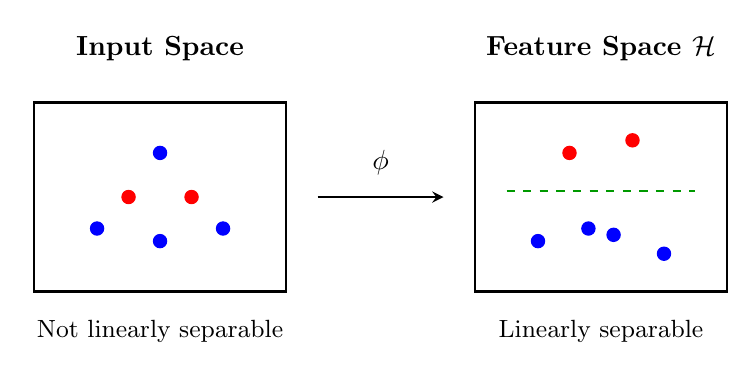
\begin{tikzpicture}[>=stealth, scale=0.8]
        % Input space
        \begin{scope}
            \node[above] at (2, 3.5) {\textbf{Input Space}};
            \draw[thick] (0,0) rectangle (4,3);

            % Non-linearly separable points
            \filldraw[red] (1.5, 1.5) circle (3pt);
            \filldraw[red] (2.5, 1.5) circle (3pt);
            \filldraw[blue] (1, 1) circle (3pt);
            \filldraw[blue] (3, 1) circle (3pt);
            \filldraw[blue] (2, 2.2) circle (3pt);
            \filldraw[blue] (2, 0.8) circle (3pt);

            \node[below] at (2, -0.3) {\small Not linearly separable};
        \end{scope}

        % Arrow
        \draw[->, thick] (4.5, 1.5) -- (6.5, 1.5);
        \node[above] at (5.5, 1.7) {$\phi$};

        % Feature space
        \begin{scope}[shift={(7,0)}]
            \node[above] at (2, 3.5) {\textbf{Feature Space $\mathcal{H}$}};
            \draw[thick] (0,0) rectangle (4,3);

            % Linearly separable after mapping
            \filldraw[red] (1.5, 2.2) circle (3pt);
            \filldraw[red] (2.5, 2.4) circle (3pt);
            \filldraw[blue] (1, 0.8) circle (3pt);
            \filldraw[blue] (3, 0.6) circle (3pt);
            \filldraw[blue] (1.8, 1) circle (3pt);
            \filldraw[blue] (2.2, 0.9) circle (3pt);

            % Separating hyperplane
            \draw[thick, green!60!black, dashed] (0.5, 1.6) -- (3.5, 1.6);

            \node[below] at (2, -0.3) {\small Linearly separable};
        \end{scope}
    \end{tikzpicture}
\caption{The kernel trick: feature map $\phi$ lifts data to a space where classes become linearly separable.}
\end{figure}

\begin{example}[Common Kernels]
    Common kernel functions include:

    \begin{itemize}
        \item \textbf{Linear}: $K(x, y) = x^\top y$. Feature map is identity.

        \item \textbf{Polynomial}: $K(x, y) = (x^\top y + c)^d$. Implicitly computes all monomials up to degree $d$.

        \item \textbf{RBF/Gaussian}: $K(x, y) = \exp(-\|x - y\|^2 / 2\sigma^2)$. Infinite-dimensional feature space.

        \item \textbf{Softmax/Exponential}: $K(x, y) = \exp(x^\top y)$. This is the attention kernel!
    \end{itemize}
\end{example}

\begin{definition}[Kernel Regression]
    Given data $\{(x_i, y_i)\}_{i=1}^n$, \textbf{kernel regression} predicts at a new point $x$ by:
    \[
        \hat{f}(x) = \sum_{i=1}^{n} w_i(x) \, y_i \quad \text{where} \quad w_i(x) = \frac{K(x, x_i)}{\sum_{j=1}^n K(x, x_j)}
    \]
    This is the \textbf{Nadaraya-Watson estimator}: a weighted average of training outputs, where weights are determined by kernel similarity to the query point.
\end{definition}

\begin{remark}[Attention IS Kernel Regression]
    Self-attention is exactly Nadaraya-Watson kernel regression. Let's see why.

    \textbf{Recall what softmax does}: For a vector $z$, the softmax normalizes by the sum:
    \[
        \text{softmax}(z)_i = \frac{e^{z_i}}{\sum_{j} e^{z_j}}
    \]
    So softmax \emph{already includes} the division by the sum---that's its whole purpose!

    \textbf{Attention weights}: Applying softmax to the attention scores:
    \[
        A_{ij} = \text{softmax}_j\left(\frac{q_i^\top k_j}{\sqrt{d_k}}\right) = \frac{\exp(q_i^\top k_j / \sqrt{d_k})}{\sum_{j'} \exp(q_i^\top k_{j'} / \sqrt{d_k})}
    \]

    \textbf{This is exactly kernel regression}: If we define $K(q, k) = \exp(q^\top k / \sqrt{d_k})$, then:
    \[
        A_{ij} = \frac{K(q_i, k_j)}{\sum_{j'} K(q_i, k_{j'})}
    \]
    which matches the Nadaraya-Watson weights. The attention output is:
    \[
        \text{output}_i = \sum_j A_{ij} v_j = \sum_j \frac{K(q_i, k_j)}{\sum_{j'} K(q_i, k_{j'})} v_j
    \]

    \textbf{Interpretation}:
    \begin{itemize}
        \item Query $q_i$ = the point where we want to predict
        \item Keys $k_j$ = the ``locations'' of data points
        \item Values $v_j$ = the ``outputs'' at those locations
        \item $K(q_i, k_j)$ = similarity between query and key (unnormalized)
        \item $A_{ij}$ = normalized similarity (weights sum to 1)
    \end{itemize}
\end{remark}

\begin{figure}[h]
\centering
    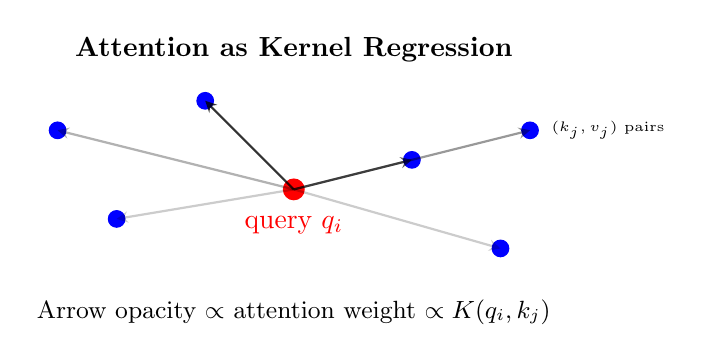
\begin{tikzpicture}[>=stealth, scale=0.75]
        % Kernel regression view
        \node[above] at (5, 4) {\textbf{Attention as Kernel Regression}};

        % Query point
        \filldraw[red] (5, 2) circle (5pt);
        \node[below, red] at (5, 1.7) {query $q_i$};

        % Key-value pairs
        \foreach \x/\y/\l in {1/3/1, 2/1.5/2, 3.5/3.5/3, 7/2.5/4, 8.5/1/5, 9/3/6} {
            \filldraw[blue] (\x, \y) circle (4pt);
        }
        \node[right, font=\tiny] at (9.2, 3) {$(k_j, v_j)$ pairs};

        % Kernel similarities (arrows with weights)
        \draw[->, thick, opacity=0.3] (5, 2) -- (1, 3);
        \draw[->, thick, opacity=0.2] (5, 2) -- (2, 1.5);
        \draw[->, thick, opacity=0.8] (5, 2) -- (3.5, 3.5);
        \draw[->, thick, opacity=0.6] (5, 2) -- (7, 2.5);
        \draw[->, thick, opacity=0.2] (5, 2) -- (8.5, 1);
        \draw[->, thick, opacity=0.4] (5, 2) -- (9, 3);

        \node[below] at (5, 0.3) {\small Arrow opacity $\propto$ attention weight $\propto K(q_i, k_j)$};
    \end{tikzpicture}
\caption{Attention as kernel regression: query retrieves a weighted average of values based on kernel similarity to keys.}
\end{figure}

\begin{remark}[What Breaks vs Classical Kernels]
    Classical RKHS (Reproducing Kernel Hilbert Space) kernels satisfy:
    \begin{enumerate}
        \item \textbf{Fixed feature map}: $K(x, y) = \phi(x)^\top \phi(y)$ for some fixed $\phi$
        \item \textbf{Symmetry}: $K(x, y) = K(y, x)$
        \item \textbf{Positive definiteness}: The Gram matrix is always PSD
    \end{enumerate}

    Self-attention \textbf{violates} these:
    \begin{itemize}
        \item \textbf{Data-dependent features}: $q_i = W_Q x_i$ and $k_j = W_K x_j$ depend on the data
        \item \textbf{Asymmetric}: $K(q_i, k_j) \neq K(q_j, k_i)$ because $W_Q \neq W_K$
        \item \textbf{Learned projections}: The ``kernel'' changes during training
    \end{itemize}

    The kernel interpretation is thus an \textbf{analogy}, not an equivalence.
\end{remark}

\begin{figure}[h]
\centering
    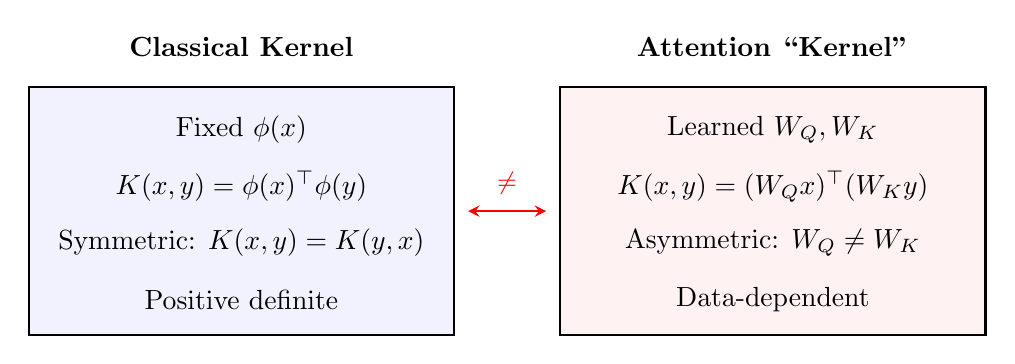
\begin{tikzpicture}[>=stealth, scale=0.9]
        % Classical kernel
        \begin{scope}
            \node[above] at (3, 3.8) {\textbf{Classical Kernel}};
            \draw[thick, fill=blue!5] (0,0) rectangle (6,3.5);
            \node at (3, 2.9) {Fixed $\phi(x)$};
            \node at (3, 2.1) {$K(x,y) = \phi(x)^\top\phi(y)$};
            \node at (3, 1.3) {Symmetric: $K(x,y) = K(y,x)$};
            \node at (3, 0.5) {Positive definite};
        \end{scope}

        % Attention "kernel"
        \begin{scope}[shift={(7.5,0)}]
            \node[above] at (3, 3.8) {\textbf{Attention ``Kernel''}};
            \draw[thick, fill=red!5] (0,0) rectangle (6,3.5);
            \node at (3, 2.9) {Learned $W_Q, W_K$};
            \node at (3, 2.1) {$K(x,y) = (W_Q x)^\top(W_K y)$};
            \node at (3, 1.3) {Asymmetric: $W_Q \neq W_K$};
            \node at (3, 0.5) {Data-dependent};
        \end{scope}

        % Arrow showing difference
        \draw[<->, thick, red] (6.2, 1.75) -- (7.3, 1.75);
        \node[above, red, font=\small] at (6.75, 1.85) {$\neq$};
    \end{tikzpicture}
\caption{Classical kernels are symmetric and fixed; attention uses learned, asymmetric projections.}
\end{figure}

\begin{remark}[Why the Asymmetry Matters]
    In attention, $W_Q \neq W_K$ creates an \textbf{asymmetric} relationship:
    \begin{itemize}
        \item ``How much does token A attend to token B?'' $\neq$ ``How much does B attend to A?''
        \item This is semantically meaningful: ``the cat sat on the mat'' --- ``cat'' should attend to ``sat'' (its verb), but ``sat'' should attend to ``cat'' (its subject) for different reasons.
    \end{itemize}

    If we forced $W_Q = W_K$ (symmetric attention), we would lose this expressivity.
\end{remark}

\begin{remark}[Why the Kernel Interpretation Matters]
    Given that attention is \textbf{not} a proper kernel method, why study this connection?

    \begin{enumerate}
        \item \textbf{Linear Attention and Efficiency}: The kernel view directly enables efficient $O(n)$ attention variants. If we decompose $K(q, k) = \phi(q)^\top \phi(k)$, then:
        \[
            \text{Attention}(q_i) = \frac{\sum_j \phi(q_i)^\top \phi(k_j) v_j}{\sum_j \phi(q_i)^\top \phi(k_j)} = \frac{\phi(q_i)^\top \sum_j \phi(k_j) v_j^\top}{\phi(q_i)^\top \sum_j \phi(k_j)}
        \]
        The sums $\sum_j \phi(k_j) v_j^\top$ and $\sum_j \phi(k_j)$ can be computed \textbf{once} and reused for all queries---this is $O(n)$ instead of $O(n^2)$.

        \item \textbf{Expressivity Analysis}: Kernel methods have well-studied approximation theory. The kernel view helps us understand what functions attention can learn (e.g., attention is a universal approximator of continuous permutation-equivariant functions on compact domains).

        \item \textbf{Implicit Feature Spaces}: Thinking of $q^\top k$ as a kernel suggests attention operates in an implicit feature space---the model learns \textbf{what similarity means} through $W_Q, W_K$ rather than hardcoding it.

        \item \textbf{Connection to Other Architectures}: The kernel view unifies attention with:
        \begin{itemize}
            \item Nadaraya-Watson regression (statistics)
            \item Graph neural networks (message passing)
            \item Memory networks (soft addressing)
        \end{itemize}
    \end{enumerate}

    The kernel analogy is imperfect but productive: it provides both practical algorithms (linear attention) and theoretical insights (expressivity, generalization).
\end{remark}

% ============================================================
\section{Positional Encodings and Length Generalization}

\begin{definition}[Positional Encoding]
    Since attention is permutation-equivariant, we must inject position information. Common approaches:

    \begin{itemize}
        \item \textbf{Absolute (Learned)}: Add learned vectors $p_i$ to each position:
        \[
            x_i \leftarrow x_i + p_i, \quad p_i \in \mathbb{R}^d \text{ learned}
        \]

        \item \textbf{Absolute (Sinusoidal)}:
        \[
            p_{i,2k} = \sin(i / 10000^{2k/d}), \quad p_{i,2k+1} = \cos(i / 10000^{2k/d})
        \]

        \item \textbf{Relative}: Attention score depends on $i - j$:
        \[
            A_{ij} \propto \exp\left(\frac{q_i^\top k_j + q_i^\top r_{i-j}}{\sqrt{d_k}}\right)
        \]

        \item \textbf{RoPE} (Rotary Position Embedding): Rotate query/key vectors by position-dependent angles:
        \[
            q_i \leftarrow R_{\theta_i} q_i, \quad k_j \leftarrow R_{\theta_j} k_j
        \]
        where $R_\theta$ is a rotation matrix. Then $q_i^\top k_j$ depends on $i - j$.
    \end{itemize}
\end{definition}

\begin{remark}[Sinusoidal Encoding: Why 10000?]
    The sinusoidal encoding uses wavelengths forming a geometric progression from $2\pi$ to $10000 \cdot 2\pi$:
    \[
        \text{wavelength}_k = 2\pi \cdot 10000^{2k/d}
    \]

    The base 10000 was chosen so that:
    \begin{itemize}
        \item \textbf{Low dimensions} ($k \approx 0$): wavelength $\approx 2\pi$, changes every position (captures fine-grained position)
        \item \textbf{High dimensions} ($k \approx d/2$): wavelength $\approx 2\pi \cdot 10000$, changes slowly (captures coarse position)
        \item \textbf{Coverage}: For sequences up to 10000 tokens, each dimension contributes meaningfully
    \end{itemize}

    The value 10000 is somewhat arbitrary---it just needs to be larger than the maximum expected sequence length. The key insight is the \textbf{geometric progression}: each dimension encodes position at a different frequency, like binary digits of a number.

    \begin{figure}[h]
    \centering
    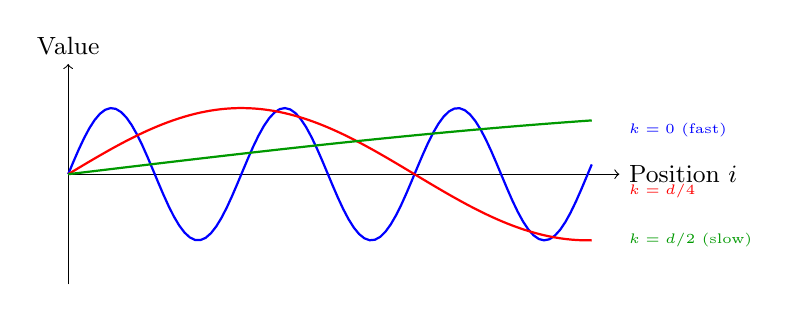
\begin{tikzpicture}[scale=0.7]
        \draw[->] (0, 0) -- (10, 0) node[right] {\small Position $i$};
        \draw[->] (0, -2) -- (0, 2) node[above] {\small Value};

        % High frequency (low dimension)
        \draw[blue, thick, domain=0:9.5, samples=100] plot (\x, {1.2*sin(2*\x r)});
        \node[blue, right] at (10, 0.8) {\tiny $k=0$ (fast)};

        % Medium frequency
        \draw[red, thick, domain=0:9.5, samples=100] plot (\x, {1.2*sin(0.5*\x r)});
        \node[red, right] at (10, -0.3) {\tiny $k=d/4$};

        % Low frequency (high dimension)
        \draw[green!60!black, thick, domain=0:9.5, samples=100] plot (\x, {1.2*sin(0.1*\x r)});
        \node[green!60!black, right] at (10, -1.2) {\tiny $k=d/2$ (slow)};
    \end{tikzpicture}
    \caption{Sinusoidal encodings: different dimensions oscillate at different frequencies.}
    \end{figure}
\end{remark}

\begin{remark}[Sinusoidal vs Learned: Historical Context]
    The original Transformer paper (Vaswani et al., 2017) proposed sinusoidal encodings for several reasons:
    \begin{enumerate}
        \item \textbf{Length extrapolation}: Sinusoidal functions are defined for any position, while learned embeddings require a fixed maximum length
        \item \textbf{Relative position}: $\sin(a+b)$ and $\cos(a+b)$ can be expressed as linear combinations of $\sin(a), \cos(a), \sin(b), \cos(b)$, so $p_{i+k}$ is a linear function of $p_i$---this allows the model to learn relative positions
        \item \textbf{No additional parameters}: Saves memory and training compute
        \item \textbf{Inductive bias}: Smooth variation between positions encourages similar treatment of nearby tokens
    \end{enumerate}

    However, the same paper showed learned embeddings performed comparably. Modern models typically use:
    \begin{itemize}
        \item \textbf{Learned absolute}: BERT, GPT-2 (simple, works well for fixed context)
        \item \textbf{RoPE}: LLaMA, GPT-NeoX (relative, better length generalization)
        \item \textbf{ALiBi}: Some models (linear bias, no learned parameters)
    \end{itemize}

    Sinusoidal encodings are now mostly historical---they demonstrated key principles but learned/RoPE methods dominate in practice.
\end{remark}

\begin{remark}[Why Absolute Encodings Fail at Length Generalization]
    With absolute positional encodings:
    \begin{itemize}
        \item The model learns position-specific patterns: ``position 5 often has verbs''
        \item At position 1000 (unseen in training), the model encounters novel embeddings
        \item The attention patterns learned for positions 1--512 don't transfer
    \end{itemize}

    The fundamental issue: \textbf{absolute positions encode ``where am I''} rather than \textbf{``how far apart are we''}.
\end{remark}

\begin{figure}[h]
\centering
    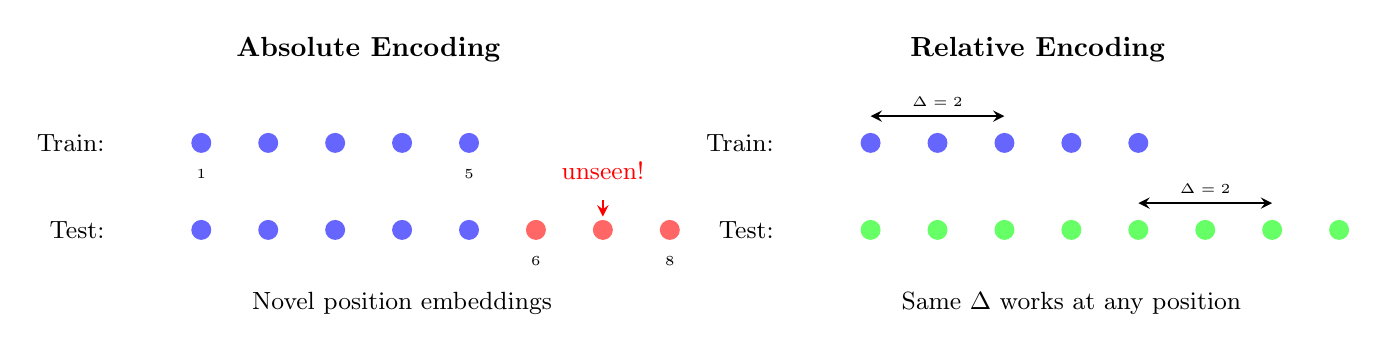
\begin{tikzpicture}[>=stealth, scale=0.85]
        % Absolute encoding problem
        \begin{scope}
            \node at (3.5, 4.2) {\textbf{Absolute Encoding}};

            % Training row
            \node[left, font=\small] at (-0.3, 2.8) {Train:};
            \foreach \i in {1,...,5} {
                \filldraw[blue!60] (\i*1, 2.8) circle (4pt);
            }
            \node[below, font=\tiny] at (1, 2.55) {1};
            \node[below, font=\tiny] at (5, 2.55) {5};

            % Test row
            \node[left, font=\small] at (-0.3, 1.5) {Test:};
            \foreach \i in {1,...,5} {
                \filldraw[blue!60] (\i*1, 1.5) circle (4pt);
            }
            \foreach \i in {6,...,8} {
                \filldraw[red!60] (\i*1, 1.5) circle (4pt);
            }
            \node[below, font=\tiny] at (6, 1.25) {6};
            \node[below, font=\tiny] at (8, 1.25) {8};
            \node[above, font=\small, red] at (7, 2.1) {unseen!};
            \draw[->, red, thick] (7, 1.95) -- (7, 1.7);

            \node at (4, 0.4) {\small Novel position embeddings};
        \end{scope}

        % Relative encoding solution
        \begin{scope}[shift={(10,0)}]
            \node at (3.5, 4.2) {\textbf{Relative Encoding}};

            % Training row
            \node[left, font=\small] at (-0.3, 2.8) {Train:};
            \foreach \i in {1,...,5} {
                \filldraw[blue!60] (\i*1, 2.8) circle (4pt);
            }
            \draw[<->, thick] (1, 3.2) -- (3, 3.2);
            \node[above, font=\tiny] at (2, 3.2) {$\Delta=2$};

            % Test row - same relative distances work
            \node[left, font=\small] at (-0.3, 1.5) {Test:};
            \foreach \i in {1,...,8} {
                \filldraw[green!60] (\i*1, 1.5) circle (4pt);
            }
            \draw[<->, thick] (5, 1.9) -- (7, 1.9);
            \node[above, font=\tiny] at (6, 1.9) {$\Delta=2$};

            \node at (4, 0.4) {\small Same $\Delta$ works at any position};
        \end{scope}
    \end{tikzpicture}
\caption{Absolute encodings fail on unseen positions; relative encodings generalize by encoding distances.}
\end{figure}

\begin{remark}[What Positional Encodings Cannot Fix]
    Even with perfect relative encodings, length generalization can fail because:
    \begin{enumerate}
        \item \textbf{Attention capacity}: With $n$ positions and fixed heads, each position can only meaningfully attend to $O(1)$ or $O(\log n)$ other positions effectively
        \item \textbf{Distribution shift}: Longer sequences have different statistical properties (more repeated patterns, different frequency distributions)
        \item \textbf{Algorithmic complexity}: Some tasks require $O(n)$ sequential steps, but transformers have $O(1)$ depth
        \item \textbf{Training signal}: The model was optimized for short sequences; the loss landscape for long sequences may be different
    \end{enumerate}
\end{remark}

% ============================================================
\section{Induction Heads}

\begin{definition}[Induction Head]
    An \textbf{induction head} is a two-attention-head circuit that implements pattern completion:
    \[
        [A][B] \cdots [A] \to [B]
    \]
    If the model has seen ``$[A][B]$'' earlier in context, and now sees ``$[A]$'', it predicts ``$[B]$''.
\end{definition}

\begin{remark}[Induction Head Mechanism]
    The circuit requires two heads working together:

    \textbf{Head 1 (Previous Token Head)}: Copies information from position $i-1$ to position $i$. Each token ``knows'' what came before it.

    \textbf{Head 2 (Induction Head)}: At position $n$, attends to positions where the \emph{previous token} matches the current token. Then copies what came \emph{after} that match.
\end{remark}

\begin{figure}[h]
\centering
    \begin{tikzpicture}[>=stealth, scale=0.9]
        % Sequence
        \node at (-1.5, 0) {\small Sequence:};
        \foreach \i/\t in {0/A, 1/B, 2/C, 3/D, 4/A, 5/?} {
            \node[draw, minimum width=0.8cm, minimum height=0.8cm] (t\i) at (\i*1.2, 0) {\t};
        }

        % Step 1: Previous token head (above)
        \node at (0.6, 2.8) {\textbf{Step 1}};
        \draw[->, thick, blue] (t0.north) to[bend left=50] (t1.north);
        \node[blue, font=\small] at (0.6, 1.8) {copies ``A''};
        \node[blue, font=\tiny] at (1.2, 1.3) {$\downarrow$};
        \node[blue, font=\tiny] at (1.2, 1.0) {B knows};
        \node[blue, font=\tiny] at (1.2, 0.7) {``A before''};

        % Step 2: Induction head (below)
        \node at (3.5, -2.5) {\textbf{Step 2}};
        \draw[->, thick, red, dashed] (t4.south) to[bend right=40] (t1.south);
        \node[red, font=\tiny] at (3, -1.5) {match: ``A before me''};
        \node[red, font=\tiny] at (3, -1.8) {= ``A before B''};

        \draw[->, thick, green!60!black] (t1.south) .. controls (2.5,-1.8) and (4.5,-1.8) .. (t5.south);
        \node[green!60!black, font=\small] at (5, -1.5) {copy B};

        % Result
        \node[right=0.3cm of t5, font=\small] {$\to$ B};
    \end{tikzpicture}
\caption{Induction head circuit: (1) previous token head copies A to B's residual; (2) induction head matches and copies.}
\end{figure}

\begin{remark}[Why Induction Heads Emerge Reliably]
    Induction heads appear consistently in transformers because:
    \begin{enumerate}
        \item \textbf{Gradient signal}: Next-token prediction heavily rewards copying patterns. When ``AB...A'' appears, predicting ``B'' gives strong gradient signal.

        \item \textbf{Simplicity}: The induction circuit is one of the simplest useful computations attention can learn. It requires only:
        \begin{itemize}
            \item Matching (via $QK^\top$)
            \item Copying (via $V$ projection)
        \end{itemize}

        \item \textbf{Weight sharing}: The same attention weights apply at all positions, so learning induction for one pattern generalizes.

        \item \textbf{Phase transition}: Anthropic observed a sharp ``phase change'' where induction heads form suddenly during training, suggesting they represent a qualitative capability jump.
    \end{enumerate}
\end{remark}

\begin{remark}[Are Induction Heads Inevitable?]
    \textbf{Largely yes}, given:
    \begin{itemize}
        \item Next-token prediction objective
        \item Sufficient depth ($\geq 2$ layers for the two-head circuit)
        \item Repeated patterns in training data
    \end{itemize}

    \textbf{What might prevent them}:
    \begin{itemize}
        \item Single-layer transformers (cannot implement the two-head circuit)
        \item Training data with no repeated patterns
        \item Extreme regularization preventing memorization
    \end{itemize}

    In practice, induction heads are nearly universal in trained transformers.
\end{remark}

% ============================================================
\section{Attention vs MLP: Routing vs Transformation}

\begin{remark}[Functional Separation]
    A useful mental model:
    \begin{itemize}
        \item \textbf{Attention}: ``Where should information flow?'' (routing, communication)
        \item \textbf{MLP}: ``What should be computed?'' (transformation, processing)
    \end{itemize}

    Attention moves information between positions; MLP processes information at each position.
\end{remark}

\begin{figure}[h]
\centering
    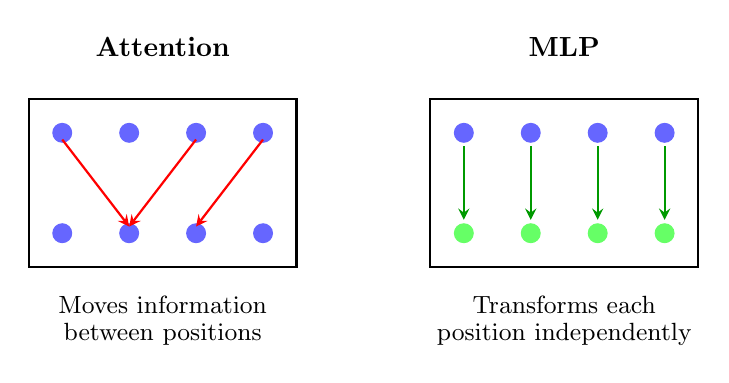
\begin{tikzpicture}[>=stealth, scale=0.85]
        % Attention
        \begin{scope}
            \node[above] at (2, 3) {\textbf{Attention}};
            \draw[thick] (0,0) rectangle (4,2.5);

            % Tokens
            \foreach \i in {0,...,3} {
                \filldraw[blue!60] (0.5 + \i, 2) circle (4pt);
                \filldraw[blue!60] (0.5 + \i, 0.5) circle (4pt);
            }

            % Arrows showing communication
            \draw[->, thick, red] (0.5, 1.9) -- (1.5, 0.6);
            \draw[->, thick, red] (2.5, 1.9) -- (1.5, 0.6);
            \draw[->, thick, red] (3.5, 1.9) -- (2.5, 0.6);

            \node[below] at (2, -0.3) {\small Moves information};
            \node[below] at (2, -0.7) {\small between positions};
        \end{scope}

        % MLP
        \begin{scope}[shift={(6,0)}]
            \node[above] at (2, 3) {\textbf{MLP}};
            \draw[thick] (0,0) rectangle (4,2.5);

            % Tokens - independent processing
            \foreach \i in {0,...,3} {
                \filldraw[blue!60] (0.5 + \i, 2) circle (4pt);
                \draw[->, thick, green!60!black] (0.5 + \i, 1.8) -- (0.5 + \i, 0.7);
                \filldraw[green!60] (0.5 + \i, 0.5) circle (4pt);
            }

            \node[below] at (2, -0.3) {\small Transforms each};
            \node[below] at (2, -0.7) {\small position independently};
        \end{scope}
    \end{tikzpicture}
\caption{Attention routes information across positions; MLP processes each position independently.}
\end{figure}

\begin{remark}[Can Each Simulate the Other?]
    \textbf{Can MLP simulate attention?} Not efficiently:
    \begin{itemize}
        \item MLP is position-wise; it cannot compare tokens at different positions
        \item To simulate attention, MLP would need $O(n^2)$ parameters for sequence length $n$
        \item Attention achieves cross-position comparison with $O(d^2)$ parameters (independent of $n$)
    \end{itemize}

    \textbf{Can attention simulate MLP?} Partially:
    \begin{itemize}
        \item Attention can implement some nonlinear functions via softmax
        \item But MLP's element-wise nonlinearity over $d_{\text{ff}}$ dimensions is hard to match
        \item Attention is fundamentally about weighted averaging, not arbitrary transformations
    \end{itemize}

    \textbf{Conclusion}: The components are complementary, not interchangeable.
\end{remark}

\begin{remark}[Formal Perspective]
    Consider the computation graph:
    \begin{itemize}
        \item \textbf{Attention}: Implements a data-dependent sparse graph over positions. The ``sparsity'' is soft (via softmax).
        \item \textbf{MLP}: Implements a dense, fixed computation at each node.
    \end{itemize}

    This separation resembles message-passing neural networks:
    \begin{itemize}
        \item Attention = message passing (aggregate from neighbors)
        \item MLP = node update (transform aggregated information)
    \end{itemize}
\end{remark}

% ============================================================
\section{In-Context Learning}

\begin{definition}[In-Context Learning (ICL)]
    \textbf{In-context learning} is the ability of a model to learn new tasks from examples provided in the prompt, without updating parameters:
    \[
        \text{prompt} = [\text{example}_1, \text{example}_2, \ldots, \text{example}_k, \text{query}]
    \]
    The model produces the correct answer to the query by ``learning'' from the examples.
\end{definition}

\begin{remark}[Competing Explanations]
    Three main theories attempt to explain ICL:

    \textbf{1. Implicit Bayesian Inference}:
    \begin{itemize}
        \item The model implicitly maintains a posterior over ``tasks'' or ``functions''
        \item Examples update this posterior; the query is answered by the posterior predictive
        \item Formally: $p(y | \text{query}, \text{examples}) = \int p(y | \text{query}, f) p(f | \text{examples}) df$
    \end{itemize}

    \textbf{2. Amortized Meta-Learning}:
    \begin{itemize}
        \item During pretraining, the model learns a meta-algorithm for learning
        \item The forward pass implements gradient descent or a similar learning algorithm
        \item ICL is ``learning to learn'' compressed into weights
    \end{itemize}

    \textbf{3. Pattern Matching in Embedding Space}:
    \begin{itemize}
        \item No true ``learning'' occurs; the model retrieves similar patterns from training
        \item Examples activate relevant ``task vectors'' in embedding space
        \item ICL is sophisticated retrieval, not inference
    \end{itemize}
\end{remark}

\begin{figure}[h]
\centering
    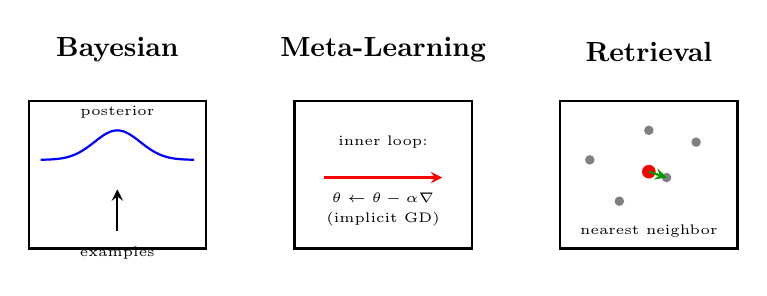
\begin{tikzpicture}[>=stealth, scale=0.75]
        % Theory 1: Bayesian
        \begin{scope}
            \node[above, font=\bfseries] at (1.5, 3) {Bayesian};
            \draw[thick] (0,0) rectangle (3,2.5);
            \draw[thick, blue] plot[smooth, domain=0.2:2.8] (\x, {1.5 + 0.5*exp(-(\x-1.5)^2/0.3)});
            \node[font=\tiny] at (1.5, 2.3) {posterior};
            \draw[->, thick] (1.5, 0.3) -- (1.5, 1);
            \node[below, font=\tiny] at (1.5, 0.2) {examples};
        \end{scope}

        % Theory 2: Meta-learning
        \begin{scope}[shift={(4.5,0)}]
            \node[above, font=\bfseries] at (1.5, 3) {Meta-Learning};
            \draw[thick] (0,0) rectangle (3,2.5);
            \node[font=\tiny] at (1.5, 1.8) {inner loop:};
            \draw[->, thick, red] (0.5, 1.2) -- (2.5, 1.2);
            \node[below, font=\tiny] at (1.5, 1.1) {$\theta \leftarrow \theta - \alpha \nabla$};
            \node[font=\tiny] at (1.5, 0.5) {(implicit GD)};
        \end{scope}

        % Theory 3: Retrieval
        \begin{scope}[shift={(9,0)}]
            \node[above, font=\bfseries] at (1.5, 3) {Retrieval};
            \draw[thick] (0,0) rectangle (3,2.5);
            % Embedding space with points
            \foreach \x/\y in {0.5/1.5, 1/0.8, 1.8/1.2, 2.3/1.8, 1.5/2} {
                \filldraw[gray] (\x, \y) circle (2pt);
            }
            \filldraw[red] (1.5, 1.3) circle (3pt);
            \draw[->, thick, green!60!black] (1.5, 1.3) -- (1.8, 1.2);
            \node[font=\tiny] at (1.5, 0.3) {nearest neighbor};
        \end{scope}
    \end{tikzpicture}
\caption{Three theories of in-context learning: Bayesian inference, implicit meta-learning, and pattern retrieval.}
\end{figure}

\begin{remark}[Falsifying Each Theory]
    \textbf{To falsify Bayesian inference}:
    \begin{itemize}
        \item Show ICL performance doesn't improve with more examples (Bayesian should converge)
        \item Show ICL fails with shuffled examples (Bayesian inference is permutation-invariant for i.i.d. examples)
        \item Find tasks where ICL succeeds but Bayesian inference would require exponential samples
    \end{itemize}

    \textbf{To falsify meta-learning}:
    \begin{itemize}
        \item Show ICL works for tasks never seen during pretraining (meta-learning requires task distribution)
        \item Demonstrate that attention patterns don't resemble gradient descent updates
        \item Show ICL in 1-layer models (gradient descent needs depth)
    \end{itemize}

    \textbf{To falsify pattern matching}:
    \begin{itemize}
        \item Show ICL on truly novel tasks with no pretraining analogues
        \item Demonstrate compositional generalization beyond training distribution
        \item Show ICL improves with more compute at inference (retrieval shouldn't)
    \end{itemize}
\end{remark}

\begin{remark}[Current Evidence]
    The evidence is mixed:
    \begin{itemize}
        \item Transformers \emph{can} implement gradient descent in their forward pass (supports meta-learning)
        \item ICL is sensitive to example order (against pure Bayesian inference)
        \item ICL often fails on truly out-of-distribution tasks (supports retrieval)
        \item Scaling improves ICL substantially (mechanism unclear)
    \end{itemize}

    The truth is likely a combination: transformers learn a flexible algorithm that has Bayesian-like properties, meta-learning structure, and retrieval components.
\end{remark}

% ============================================================
\section{Expressivity: Depth vs Width}

\begin{remark}[The Core Question]
    \textbf{Can a single-layer transformer with very wide attention simulate a deep transformer?}

    Intuitively:
    \begin{itemize}
        \item More heads = more parallel computations
        \item Wider FFN = more features
        \item But can width substitute for depth?
    \end{itemize}
\end{remark}

\begin{theorem}[Width Can Simulate Depth---At Exponential Cost]
    A single-layer transformer with $O(L \cdot d^L)$ heads can simulate an $L$-layer transformer with $d$ dimensions.

    \textbf{Proof sketch}: Enumerate all possible $L$-step computations and implement each with a separate head.
\end{theorem}

\begin{remark}[Where Depth is Strictly Necessary]
    Depth provides exponential efficiency for:

    \textbf{1. Sequential Computation}:
    \begin{itemize}
        \item Tasks requiring $k$ sequential steps need $\Omega(k)$ layers
        \item Example: Composing $k$ functions $f_k \circ f_{k-1} \circ \cdots \circ f_1$
        \item Width cannot parallelize inherently sequential computation
    \end{itemize}

    \textbf{2. Iterative Refinement}:
    \begin{itemize}
        \item Many algorithms iterate: gradient descent, Newton's method, belief propagation
        \item Each iteration refines the previous output
        \item Depth = number of refinement steps
    \end{itemize}

    \textbf{3. Hierarchical Composition}:
    \begin{itemize}
        \item Recognizing ``noun phrase inside prepositional phrase inside sentence''
        \item Each layer builds higher-level abstractions
        \item Width gives more features at one level; depth gives more levels
    \end{itemize}
\end{remark}

\begin{figure}[h]
\centering
    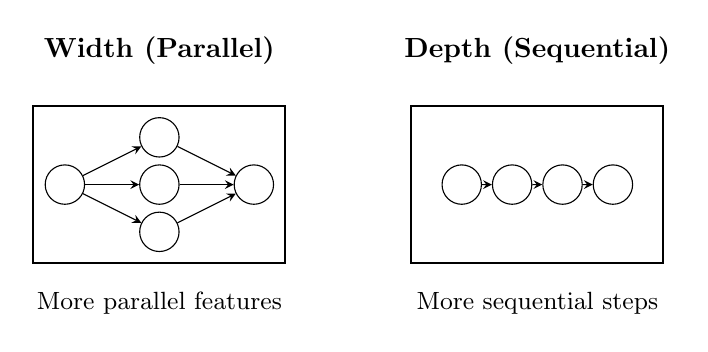
\begin{tikzpicture}[>=stealth, scale=0.8]
        % Width
        \begin{scope}
            \node[above, font=\bfseries] at (2, 3) {Width (Parallel)};
            \draw[thick] (0,0) rectangle (4,2.5);

            \node[draw, circle, minimum size=0.5cm] (i) at (0.5, 1.25) {};
            \node[draw, circle, minimum size=0.5cm] (ha) at (2, 0.5) {};
            \node[draw, circle, minimum size=0.5cm] (hb) at (2, 1.25) {};
            \node[draw, circle, minimum size=0.5cm] (hc) at (2, 2) {};
            \draw[->] (i) -- (ha);
            \draw[->] (i) -- (hb);
            \draw[->] (i) -- (hc);
            \node[draw, circle, minimum size=0.5cm] (o) at (3.5, 1.25) {};
            \draw[->] (ha) -- (o);
            \draw[->] (hb) -- (o);
            \draw[->] (hc) -- (o);

            \node[below, font=\small] at (2, -0.3) {More parallel features};
        \end{scope}

        % Depth
        \begin{scope}[shift={(6,0)}]
            \node[above, font=\bfseries] at (2, 3) {Depth (Sequential)};
            \draw[thick] (0,0) rectangle (4,2.5);

            \node[draw, circle, minimum size=0.5cm] (l1) at (0.8, 1.25) {};
            \node[draw, circle, minimum size=0.5cm] (l2) at (1.6, 1.25) {};
            \node[draw, circle, minimum size=0.5cm] (l3) at (2.4, 1.25) {};
            \node[draw, circle, minimum size=0.5cm] (l4) at (3.2, 1.25) {};

            \draw[->] (l1) -- (l2);
            \draw[->] (l2) -- (l3);
            \draw[->] (l3) -- (l4);

            \node[below, font=\small] at (2, -0.3) {More sequential steps};
        \end{scope}
    \end{tikzpicture}
\caption{Width enables parallel feature computation; depth enables sequential refinement.}
\end{figure}

\begin{remark}[Formal Results]
    \textbf{Circuit complexity}: Transformers with $L$ layers can compute functions in $\mathsf{TC}^0$ (constant-depth threshold circuits) with $O(L)$ ``rounds'' of adaptive computation.

    \textbf{Separation}: There exist functions computable by depth-$L$ transformers that require width $\exp(\Omega(L))$ for depth-1 transformers.

    \textbf{Practical implication}: For most tasks, moderate depth (12--96 layers) with moderate width is more efficient than extreme width with minimal depth.
\end{remark}

% ============================================================
\section{Information Bottlenecks in Attention}

\begin{remark}[The Bottleneck]
    With $H$ attention heads and hidden dimension $d$, self-attention imposes a bottleneck:

    \textbf{Per-head capacity}: Each head has dimension $d_k = d/H$. The attention matrix $A \in \mathbb{R}^{n \times n}$ can encode at most $n \cdot d_k$ bits of information about which positions to attend.

    \textbf{Rank constraint}: The attention output for head $h$ is:
    \[
        \text{head}_h = A_h V_h \in \mathbb{R}^{n \times d_v}
    \]
    where $\text{rank}(A_h V_h) \leq \min(n, d_v, \text{rank}(A_h))$.
\end{remark}

\begin{remark}[Scaling with Sequence Length]
    As sequence length $n$ grows:

    \textbf{Attention is $O(n^2)$}: Computing $QK^\top$ requires $O(n^2)$ operations and memory.

    \textbf{But information per position is $O(1)$}: Each position receives a $d$-dimensional vector, regardless of $n$. Long-range dependencies must be compressed into this fixed capacity.

    \textbf{Effective context}: Empirically, attention weights concentrate on $O(1)$ or $O(\log n)$ positions. Most positions receive negligible attention.
\end{remark}

\begin{figure}[h]
\centering
    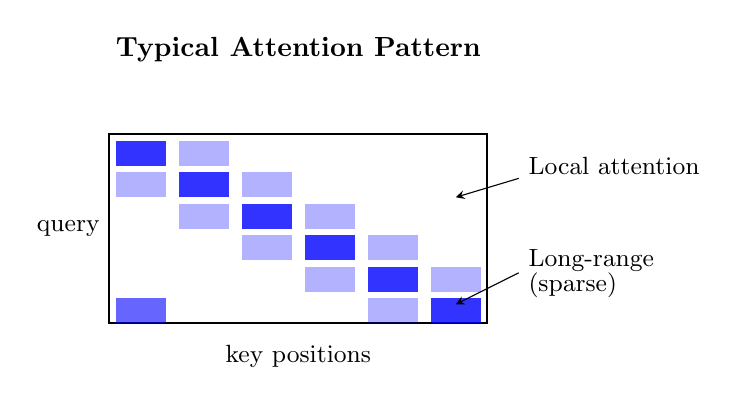
\begin{tikzpicture}[>=stealth, scale=0.8]
        % Attention pattern visualization
        \node[above] at (3, 4) {\textbf{Typical Attention Pattern}};

        \draw[thick] (0,0) rectangle (6,3);

        % Sparse attention pattern
        \foreach \i in {0,...,5} {
            \foreach \j in {0,...,5} {
                \pgfmathsetmacro{\val}{
                    (\i==\j) * 0.8 +
                    (abs(\i-\j)==1) * 0.3 +
                    ((\i==5) && (\j==0)) * 0.6
                }
                \fill[blue, opacity=\val] (\j+0.1, 2.9-\i*0.5) rectangle (\j+0.9, 2.5-\i*0.5);
            }
        }

        % Labels
        \node[left, font=\small] at (0, 1.5) {query};
        \node[below, font=\small] at (3, -0.2) {key positions};

        % Annotation
        \node[right, font=\small] at (6.5, 2.5) {Local attention};
        \draw[->] (6.5, 2.3) -- (5.5, 2);

        \node[right, font=\small] at (6.5, 1) {Long-range};
        \node[right, font=\small] at (6.5, 0.6) {(sparse)};
        \draw[->] (6.5, 0.8) -- (5.5, 0.3);
    \end{tikzpicture}
\caption{Attention concentrates on diagonal (local) with sparse long-range connections.}
\end{figure}

\begin{remark}[Information-Theoretic View]
    Consider the mutual information between position $i$'s output and distant position $j$'s input:
    \[
        I(\text{output}_i; \text{input}_j) \leq H(\text{attention weights on } j) \leq \log_2(\text{precision})
    \]

    With float16 attention weights, each position can communicate at most $\sim 16$ bits per head to any other position. For a sequence of length 10,000, this is a severe bottleneck.

    \textbf{Implication}: Transformers must learn to route important information through multiple hops or compress it efficiently. This is why intermediate ``summary'' tokens and hierarchical attention patterns emerge.
\end{remark}

% ============================================================
\section{Optimization Landscape}

\begin{remark}[The Mystery]
    Transformers are highly non-convex with billions of parameters, yet:
    \begin{itemize}
        \item They train reliably with SGD/Adam
        \item Loss decreases smoothly (no catastrophic failures)
        \item Different random seeds converge to similar performance
    \end{itemize}

    Why are they ``easy'' to optimize?
\end{remark}

\begin{remark}[Role of Residual Connections]
    Beyond gradient flow, residuals shape the loss landscape:

    \textbf{1. Linear path at initialization}:
    \begin{itemize}
        \item At init, layer outputs are small (weights near zero)
        \item The network is approximately $x + \epsilon \cdot F(x) \approx x$
        \item The loss landscape is nearly convex initially
    \end{itemize}

    \textbf{2. Gradual nonlinearity}:
    \begin{itemize}
        \item As training progresses, $F(x)$ grows
        \item Nonlinearity increases gradually
        \item The optimization ``follows'' a path from convex to non-convex
    \end{itemize}

    \textbf{3. Ensemble effect}:
    \begin{itemize}
        \item With residuals, a depth-$L$ network has $2^L$ paths (include/exclude each layer)
        \item This implicit ensemble smooths the loss landscape
    \end{itemize}
\end{remark}

\begin{figure}[h]
\centering
    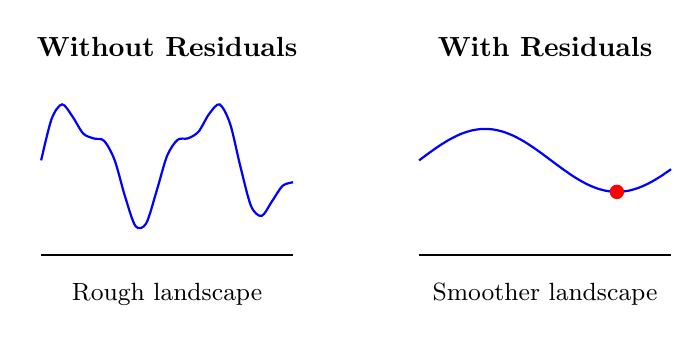
\begin{tikzpicture}[>=stealth, scale=0.8]
        % Without residuals
        \begin{scope}
            \node[above] at (2, 3) {\textbf{Without Residuals}};
            \draw[thick] (0,0) -- (4,0);
            \draw[thick, blue] plot[smooth, domain=0:4] (\x, {1.5 + 0.8*sin(3*\x r) + 0.3*sin(7*\x r)});
            \node[below] at (2, -0.3) {\small Rough landscape};
        \end{scope}

        % With residuals
        \begin{scope}[shift={(6,0)}]
            \node[above] at (2, 3) {\textbf{With Residuals}};
            \draw[thick] (0,0) -- (4,0);
            \draw[thick, blue] plot[smooth, domain=0:4] (\x, {1.5 + 0.5*sin(1.5*\x r)});
            \node[below] at (2, -0.3) {\small Smoother landscape};

            % Minimum
            \filldraw[red] (3.14, 1) circle (3pt);
        \end{scope}
    \end{tikzpicture}
\caption{Residual connections smooth the loss landscape, making optimization easier.}
\end{figure}

\begin{remark}[Role of Layer Normalization]
    LayerNorm provides:

    \textbf{1. Scale invariance}:
    \begin{itemize}
        \item Activations are normalized to unit variance
        \item Gradient magnitudes are controlled regardless of layer
    \end{itemize}

    \textbf{2. Implicit learning rate adaptation}:
    \begin{itemize}
        \item LayerNorm's Jacobian depends on activation statistics
        \item This creates an adaptive, per-neuron learning rate
    \end{itemize}

    \textbf{3. Loss landscape conditioning}:
    \begin{itemize}
        \item The Hessian eigenvalues are bounded more tightly
        \item This allows larger learning rates without divergence
    \end{itemize}
\end{remark}

\begin{remark}[Additional Factors]
    \begin{itemize}
        \item \textbf{Overparameterization}: More parameters than needed creates many equivalent minima
        \item \textbf{Data scale}: Large datasets provide consistent gradients (low variance)
        \item \textbf{Attention sparsity}: Attention weights are soft-sparse, reducing effective nonlinearity
        \item \textbf{Adam optimizer}: Adaptive learning rates handle different parameter scales
    \end{itemize}
\end{remark}

% ============================================================
\section{Length Generalization Failures}

\begin{remark}[The Problem]
    Transformers often fail to generalize to longer sequences, even when:
    \begin{itemize}
        \item The task is algorithmically length-invariant (e.g., addition, copying)
        \item Relative position encodings are used
        \item The model has ``enough'' capacity
    \end{itemize}
\end{remark}

\begin{example}[Addition Failure]
    Train a transformer on 5-digit addition:
    \[
        12345 + 67890 = 80235 \quad \checkmark
    \]
    Test on 10-digit addition:
    \[
        1234567890 + 9876543210 = ? \quad \text{(often wrong)}
    \]
    The algorithm is the same, but the model fails.
\end{example}

\begin{remark}[Causes of Length Generalization Failure]
    \textbf{1. Attention Distribution Shift}:
    \begin{itemize}
        \item With more positions, attention is spread thinner
        \item Patterns that worked with 10 positions fail with 1000
        \item Even relative encodings don't fix the attention \emph{sharpness}
    \end{itemize}

    \textbf{2. Positional Encoding Extrapolation}:
    \begin{itemize}
        \item Learned positions: unseen indices have random embeddings
        \item Sinusoidal: extrapolates but at different frequencies
        \item RoPE: better but still degrades beyond training length
    \end{itemize}

    \textbf{3. Depth Limitations}:
    \begin{itemize}
        \item Some algorithms require $O(n)$ sequential steps
        \item Transformers have $O(L)$ depth, independent of $n$
        \item Example: Checking balanced parentheses needs a ``stack'' that grows with $n$
    \end{itemize}

    \textbf{4. Training Distribution}:
    \begin{itemize}
        \item The model is optimized for short sequences
        \item Features learned for length 100 may not transfer to length 10,000
        \item The loss landscape for long sequences is different
    \end{itemize}
\end{remark}

\begin{figure}[h]
\centering
    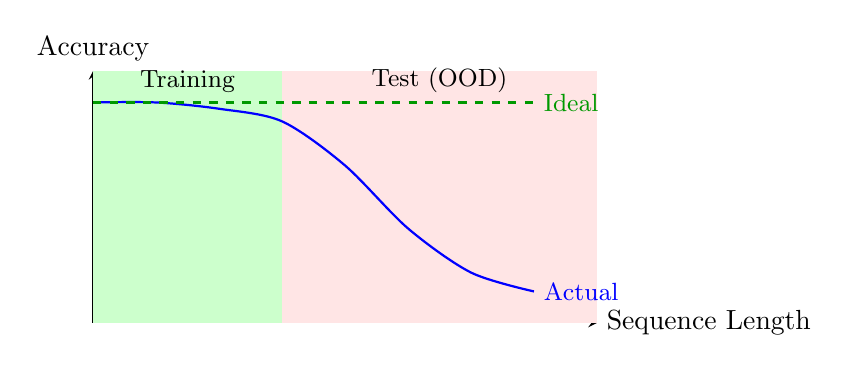
\begin{tikzpicture}[>=stealth, scale=0.8]
        % Training performance
        \draw[->] (0,0) -- (8,0) node[right] {Sequence Length};
        \draw[->] (0,0) -- (0,4) node[above] {Accuracy};

        % Training region
        \fill[green!20] (0,0) rectangle (3,4);
        \node[above] at (1.5, 3.5) {\small Training};

        % Test region
        \fill[red!10] (3,0) rectangle (8,4);
        \node[above] at (5.5, 3.5) {\small Test (OOD)};

        % Performance curve
        \draw[thick, blue] plot[smooth] coordinates {(0,3.5) (1,3.5) (2,3.4) (3,3.2) (4,2.5) (5,1.5) (6,0.8) (7,0.5)};

        % Ideal
        \draw[thick, dashed, green!60!black] (0,3.5) -- (7,3.5);
        \node[right, green!60!black, font=\small] at (7,3.5) {Ideal};

        % Actual
        \node[right, blue, font=\small] at (7,0.5) {Actual};
    \end{tikzpicture}
\caption{Length generalization failure: accuracy degrades beyond training sequence lengths.}
\end{figure}

% ============================================================
\section{Universality vs Efficiency}

\begin{theorem}[Transformer Universality]
    Transformers are universal sequence-to-sequence approximators: for any continuous function $f: \mathbb{R}^{n \times d} \to \mathbb{R}^{n \times d}$ and $\epsilon > 0$, there exists a transformer $T$ such that $\|T(X) - f(X)\| < \epsilon$ for all $X$ in a compact domain.
\end{theorem}

\begin{remark}[But At What Cost?]
    Universality says nothing about efficiency. Key questions:

    \textbf{1. Width/depth requirements}:
    \begin{itemize}
        \item Some functions require exponential width or depth
        \item Universality proofs often use $O(1/\epsilon^d)$ parameters
    \end{itemize}

    \textbf{2. Sample complexity}:
    \begin{itemize}
        \item Learning the approximation may require exponential data
        \item Existence $\neq$ learnability
    \end{itemize}
\end{remark}

\begin{remark}[Comparison with Other Architectures]
    \textbf{Transformers vs RNNs}:
    \begin{center}
        \begin{tabular}{l|cc}
            & \textbf{Transformer} & \textbf{RNN} \\
            \hline
            Parallel training & $O(1)$ depth & $O(n)$ sequential \\
            Long-range deps & $O(1)$ path length & $O(n)$ path length \\
            Memory & $O(n^2)$ attention & $O(1)$ state \\
            Sequential tasks & $O(L)$ layers & $O(n)$ natural \\
        \end{tabular}
    \end{center}

    \textbf{Transformers vs State-Space Models (SSMs)}:
    \begin{itemize}
        \item SSMs (Mamba, S4) have $O(n)$ complexity vs $O(n^2)$
        \item SSMs maintain compressed state; may lose information
        \item SSMs are better for very long sequences; worse for tasks requiring full context access
    \end{itemize}
\end{remark}

\begin{remark}[Function Classes]
    Functions efficiently representable by transformers:
    \begin{itemize}
        \item \textbf{Efficient}: Pattern matching, copying, soft retrieval, shallow reasoning
        \item \textbf{Possible but costly}: Deep recursion, arithmetic, precise counting
        \item \textbf{Likely exponential}: Arbitrary graph algorithms, general-purpose computation
    \end{itemize}

    The transformer architecture is biased toward:
    \begin{itemize}
        \item Parallel, shallow computation
        \item Soft, differentiable operations
        \item Pattern recognition over symbolic manipulation
    \end{itemize}
\end{remark}

\begin{figure}[h]
\centering
    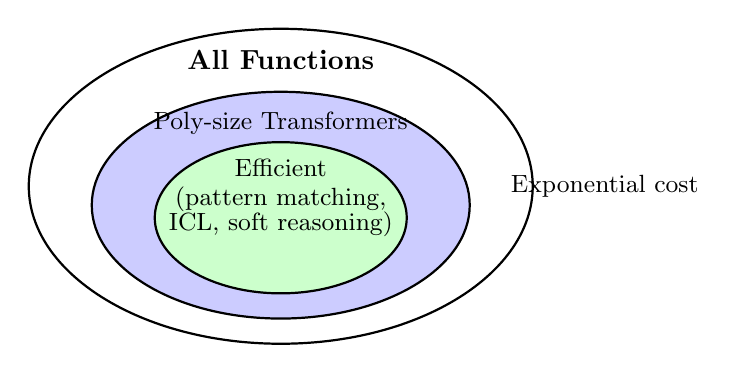
\begin{tikzpicture}[>=stealth, scale=0.8]
        % Complexity classes
        \draw[thick] (0,0) ellipse (4cm and 2.5cm);
        \node at (0, 2) {\textbf{All Functions}};

        \draw[thick, fill=blue!20] (0,-0.3) ellipse (3cm and 1.8cm);
        \node at (0, 1) {\small Poly-size Transformers};

        \draw[thick, fill=green!20] (0,-0.5) ellipse (2cm and 1.2cm);
        \node[font=\small] at (0, 0.3) {Efficient};
        \node[font=\small] at (0, -0.2) {(pattern matching,};
        \node[font=\small] at (0, -0.6) {ICL, soft reasoning)};

        % Labels outside
        \node[right] at (3.5, 0) {\small Exponential cost};
    \end{tikzpicture}
\caption{Hierarchy of function classes: transformers efficiently compute a subset of representable functions.}
\end{figure}

% ============================================================
% ============================================================
\chapter{Training Phases of Large Language Models}

Modern LLMs are trained in distinct phases, each with different objectives, data, and which parameters are updated.

\section{Overview of Training Phases}

\begin{figure}[h]
\centering
    \begin{tikzpicture}[
            box/.style={draw, rounded corners, minimum width=3.5cm, minimum height=1.2cm, align=center},
            arrow/.style={->, thick, >=stealth}
        ]
        % Boxes
        \node[box, fill=blue!15] (pre) at (0,0) {\textbf{Pretraining}\\Next-token prediction};
        \node[box, fill=orange!15] (mid) at (5,0) {\textbf{Midtraining}\\Domain adaptation};
        \node[box, fill=green!15] (post) at (10,0) {\textbf{Post-training}\\Alignment (SFT + RLHF)};

        % Arrows
        \draw[arrow] (pre) -- (mid);
        \draw[arrow] (mid) -- (post);

        % Labels below
        \node[below=0.3cm of pre, align=center, font=\small] {Trillions of tokens\\All params trained};
        \node[below=0.3cm of mid, align=center, font=\small] {Billions of tokens\\All or most params};
        \node[below=0.3cm of post, align=center, font=\small] {Millions of examples\\Often frozen/LoRA};
    \end{tikzpicture}
\caption{The three phases of LLM training: pretraining, midtraining, and post-training.}
\end{figure}

% ============================================================
\section{Pretraining}

\begin{definition}[Pretraining]
    \textbf{Pretraining} is the initial phase where the model learns general language understanding from a massive corpus using self-supervised learning.

    \textbf{Objective}: Next-token prediction (autoregressive LM):
    \[
        \mathcal{L}_{\text{pretrain}} = -\sum_{t=1}^{T} \log p_\theta(x_t | x_{<t})
    \]

    \textbf{Data}: Web crawls (Common Crawl), books, Wikipedia, code. Typically 1--15 trillion tokens.

    \textbf{Parameters}: \textbf{All parameters trained from random initialization.}
\end{definition}

\begin{remark}[What the Model Learns]
    During pretraining, the model acquires:
    \begin{itemize}
        \item \textbf{Syntax}: Grammar, sentence structure, agreement
        \item \textbf{Semantics}: Word meanings, relationships, common sense
        \item \textbf{World knowledge}: Facts, dates, named entities
        \item \textbf{Reasoning patterns}: (to some extent) logical deduction, arithmetic
    \end{itemize}
    The model is ``raw''---it completes text but doesn't follow instructions.
\end{remark}

% ============================================================
\section{Midtraining (Continued Pretraining)}

\begin{definition}[Midtraining]
    \textbf{Midtraining} extends pretraining on domain-specific data to specialize the model.

    \textbf{Objective}: Same as pretraining (next-token prediction), but on curated domain data.

    \textbf{Data}: Domain-specific corpora (medical, legal, code, scientific). Billions of tokens.
\end{definition}

\begin{remark}[Freezing During Midtraining]
    Common approaches:
    \begin{enumerate}
        \item \textbf{Full fine-tuning}: All parameters updated. Risk of catastrophic forgetting.
        \item \textbf{Freeze embeddings}: Keep token embeddings fixed; train transformer layers.
        \item \textbf{Freeze early layers}: Early layers capture syntax; freezing preserves basic patterns.
        \item \textbf{Layerwise LR decay}: Earlier layers get smaller updates.
    \end{enumerate}

    \textbf{Typical practice}: Train all parameters but with lower learning rate and mixed data.
\end{remark}

% ============================================================
\section{Post-training (Alignment)}

Post-training transforms a raw LM into an assistant that follows instructions.

\subsection{Supervised Fine-Tuning (SFT)}

\begin{definition}[Supervised Fine-Tuning]
    \textbf{SFT} trains the model on (instruction, response) pairs:
    \[
        \mathcal{L}_{\text{SFT}} = -\sum_{t=1}^{T} \log p_\theta(y_t | x, y_{<t})
    \]
    where $x$ is the instruction and $y$ is the desired response.
\end{definition}

\subsection{RLHF / Preference Optimization}

\begin{definition}[RLHF]
    \textbf{RLHF} refines the model using human preferences:
    \begin{enumerate}
        \item Train a reward model on preference data
        \item Use RL (PPO) to optimize:
              \[
                  \max_\theta \mathbb{E}_{y \sim \pi_\theta}[R(x, y)] - \beta \, D_{\mathrm{KL}}(\pi_\theta \| \pi_{\text{ref}})
              \]
    \end{enumerate}
\end{definition}

\begin{remark}[Freezing During Post-training]
    Common strategies:
    \begin{enumerate}
        \item \textbf{Full fine-tuning}: Update all parameters.
        \item \textbf{LoRA}: Freeze pretrained weights; add low-rank adapters.
        \item \textbf{Freeze embeddings}: Vocabulary unchanged; no need to update.
        \item \textbf{Freeze early layers}: Alignment affects high-level behavior (later layers).
    \end{enumerate}
\end{remark}

\begin{remark}[Summary: What Gets Frozen]
    \begin{center}
        \begin{tabular}{l|ccc}
                                     & \textbf{Pretraining} & \textbf{Midtraining} & \textbf{Post-training} \\
            \hline
            Embeddings               & Train                & Train or Freeze      & Usually Freeze         \\
            Early transformer layers & Train                & Train (lower LR)     & Often Freeze / LoRA    \\
            Late transformer layers  & Train                & Train                & Train / LoRA           \\
            LM head (unembedding)    & Train                & Train                & Train or Freeze        \\
            Layer norms              & Train                & Train                & Train                  \\
        \end{tabular}
    \end{center}
\end{remark}

% ============================================================
\section{Parameter-Efficient Fine-Tuning (PEFT)}

\begin{definition}[LoRA]
    \textbf{Low-Rank Adaptation} freezes pretrained weights $W$ and adds trainable low-rank matrices:
    \[
        h = Wx + BAx
    \]
    where $B \in \mathbb{R}^{d_{\text{out}} \times r}$, $A \in \mathbb{R}^{r \times d_{\text{in}}}$, and $r \ll \min(d_{\text{out}}, d_{\text{in}})$.

    At initialization, $B = 0$, so $BA = 0$ and output matches the frozen model.
\end{definition}

\begin{example}[LoRA Savings]
    For $W \in \mathbb{R}^{4096 \times 4096}$:
    \begin{itemize}
        \item Full: $4096^2 = 16.7$M parameters
        \item LoRA ($r=16$): $(4096 + 4096) \times 16 = 131$K parameters (0.8\%)
    \end{itemize}
\end{example}

\begin{remark}[Other PEFT Methods]
    \begin{itemize}
        \item \textbf{QLoRA}: LoRA + 4-bit quantization. Fine-tune 65B on single GPU.
        \item \textbf{Prefix Tuning}: Learn virtual tokens prepended to input.
        \item \textbf{Adapters}: Insert small trainable layers between blocks.
    \end{itemize}
\end{remark}

% ============================================================
\section{Encoder-Decoder vs Decoder-Only Architecture}

The original Transformer was designed for sequence-to-sequence tasks like translation. Modern language models use only the decoder.

\begin{definition}[Original Transformer Architecture]
    The \textbf{Attention Is All You Need} architecture has two components:
    \begin{itemize}
        \item \textbf{Encoder}: Processes the input sequence (e.g., English sentence). Uses bidirectional self-attention---each token can attend to all others.
        \item \textbf{Decoder}: Generates the output sequence (e.g., French translation). Uses causal self-attention + cross-attention to the encoder.
    \end{itemize}
\end{definition}

\begin{remark}[Cross-Attention: Q from Decoder, K/V from Encoder]
    In cross-attention:
    \[
        Q = X_{\text{dec}} W_Q, \quad K = X_{\text{enc}} W_K, \quad V = X_{\text{enc}} W_V
    \]

    Why this asymmetry?
    \begin{itemize}
        \item \textbf{Query from decoder}: ``What information do I need to generate the next target token?''
        \item \textbf{Keys from encoder}: ``Where in the source sentence is relevant information?''
        \item \textbf{Values from encoder}: ``What is the actual content to retrieve?''
    \end{itemize}

    The decoder ``asks questions'' (Q) about the encoder's representation (K, V). This allows each decoder position to selectively read from the encoded source.
\end{remark}

\begin{figure}[h]
\centering
    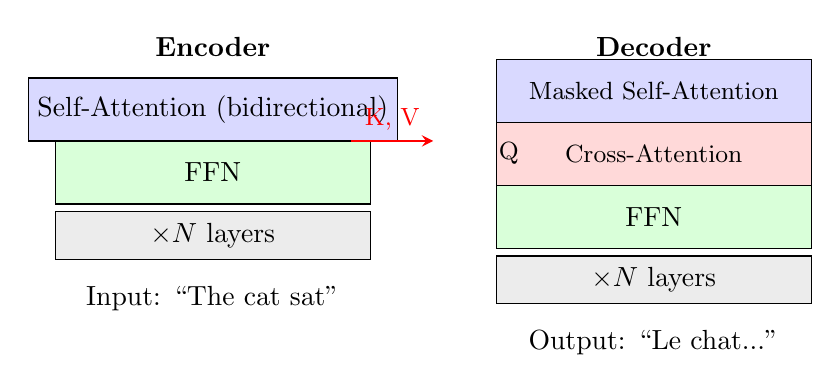
\begin{tikzpicture}[>=stealth, scale=0.8]
        % Encoder side
        \begin{scope}
            \node[font=\bfseries] at (2, 5) {Encoder};
            \node[draw, minimum width=4cm, minimum height=0.8cm, fill=blue!15] at (2, 4) {Self-Attention (bidirectional)};
            \node[draw, minimum width=4cm, minimum height=0.8cm, fill=green!15] at (2, 3) {FFN};
            \node[draw, minimum width=4cm, minimum height=0.6cm, fill=gray!15] at (2, 2) {$\times N$ layers};
            \node at (2, 1) {Input: ``The cat sat''};

            % Output K, V
            \draw[->, thick, red] (4.2, 3.5) -- (5.5, 3.5) node[midway, above] {\small K, V};
        \end{scope}

        % Decoder side
        \begin{scope}[shift={(7, 0)}]
            \node[font=\bfseries] at (2, 5) {Decoder};
            \node[draw, minimum width=4cm, minimum height=0.8cm, fill=blue!15] at (2, 4.3) {\small Masked Self-Attention};
            \node[draw, minimum width=4cm, minimum height=0.8cm, fill=red!15] at (2, 3.3) {\small Cross-Attention};
            \node at (-0.3, 3.3) {\small Q};
            \node[draw, minimum width=4cm, minimum height=0.8cm, fill=green!15] at (2, 2.3) {FFN};
            \node[draw, minimum width=4cm, minimum height=0.6cm, fill=gray!15] at (2, 1.3) {$\times N$ layers};
            \node at (2, 0.3) {Output: ``Le chat...''};
        \end{scope}
    \end{tikzpicture}
\caption{Encoder-decoder architecture: encoder provides K/V for cross-attention; decoder queries with Q.}
\end{figure}

\begin{remark}[Why Decoder-Only for Language Models?]
    Modern LLMs (GPT, LLaMA, Claude) use \textbf{decoder-only} architecture because:
    \begin{enumerate}
        \item \textbf{Unified task}: Language modeling is next-token prediction, not translation. No separate source/target.
        \item \textbf{Simplicity}: One model type, half the parameters for same depth.
        \item \textbf{Flexibility}: Same architecture handles completion, chat, reasoning.
        \item \textbf{Scaling}: Simpler architecture scales better empirically.
    \end{enumerate}

    The encoder-decoder split only makes sense when input and output are fundamentally different (translation, summarization with fixed input).
\end{remark}

\begin{definition}[Decoder-Only Architecture]
    A \textbf{decoder-only} transformer for language modeling consists of:
    \begin{enumerate}
        \item Token embedding + positional encoding
        \item $N \times$ blocks of:
        \begin{itemize}
            \item Masked (causal) multi-head self-attention
            \item Add \& LayerNorm
            \item Feed-forward network
            \item Add \& LayerNorm
        \end{itemize}
        \item Final LayerNorm
        \item Linear projection to vocabulary
        \item Softmax for next-token probabilities
    \end{enumerate}

    No encoder, no cross-attention. The model only sees past tokens.
\end{definition}

% ============================================================
\section{Attention Dimensions in Practice}

\begin{remark}[Typical Dimensions (Attention Is All You Need)]
    The original Transformer paper used:
    \begin{itemize}
        \item $d_{\text{model}} = 512$ (embedding dimension)
        \item $H = 8$ heads
        \item $d_k = d_v = d_{\text{model}} / H = 64$ per head
        \item $W_Q, W_K, W_V \in \mathbb{R}^{512 \times 64}$ for each head
        \item $W_O \in \mathbb{R}^{512 \times 512}$ (output projection)
    \end{itemize}

    The ``base'' model had $N = 6$ encoder and decoder layers. The ``big'' model used $d_{\text{model}} = 1024$, $H = 16$ heads.
\end{remark}

\begin{remark}[Why Separate $W_Q$, $W_K$, $W_V$ Instead of One Matrix?]
    One might think: since we compute $QK^\top = (XW_Q)(XW_K)^\top = X(W_Q W_K^\top)X^\top$, why not learn $W_{QK} = W_Q W_K^\top$ directly?

    The problem is dimensionality:
    \begin{itemize}
        \item $W_Q \in \mathbb{R}^{d \times d_k}$, $W_K \in \mathbb{R}^{d \times d_k}$ $\Rightarrow$ $2 d \cdot d_k$ parameters
        \item $W_{QK} = W_Q W_K^\top \in \mathbb{R}^{d \times d}$ $\Rightarrow$ $d^2$ parameters
    \end{itemize}

    For GPT-3 with $d = 12288$ and $d_k = 128$:
    \begin{itemize}
        \item Factored: $2 \times 12288 \times 128 = 3.1$M parameters
        \item Combined: $12288^2 = 151$M parameters (48$\times$ larger!)
    \end{itemize}

    The factorization is a \textbf{low-rank constraint}: we're forcing $W_{QK}$ to have rank at most $d_k$, which acts as regularization and saves massive compute/memory.
\end{remark}

\begin{remark}[Why Not $Q = K = V$?]
    If we set $W_Q = W_K = W_V$, attention becomes symmetric:
    \[
        A_{ij} = A_{ji} \quad \text{(how much $i$ attends to $j$ = how much $j$ attends to $i$)}
    \]

    This loses expressivity:
    \begin{itemize}
        \item Can't learn asymmetric relations (``subject attends to verb'' vs ``verb attends to subject'')
        \item Query-key separation lets the model learn \textbf{what to look for} (Q) separately from \textbf{what to match against} (K)
        \item Value separation lets the model learn \textbf{what information to extract} independently
    \end{itemize}

    Empirically, tied projections perform significantly worse.
\end{remark}

% ============================================================
\section{KV Cache for Efficient Inference}

During autoregressive generation, we can cache computed keys and values to avoid redundant computation.

\begin{definition}[KV Cache]
    For a decoder generating token $t+1$ given tokens $1, \ldots, t$:
    \begin{itemize}
        \item \textbf{Without cache}: Recompute $K = [k_1, \ldots, k_t, k_{t+1}]$ and $V = [v_1, \ldots, v_t, v_{t+1}]$ from scratch.
        \item \textbf{With cache}: Store $K_{\text{cache}} = [k_1, \ldots, k_t]$ and $V_{\text{cache}} = [v_1, \ldots, v_t]$. Only compute $k_{t+1}, v_{t+1}$ for the new token and append.
    \end{itemize}
\end{definition}

\begin{figure}[h]
\centering
    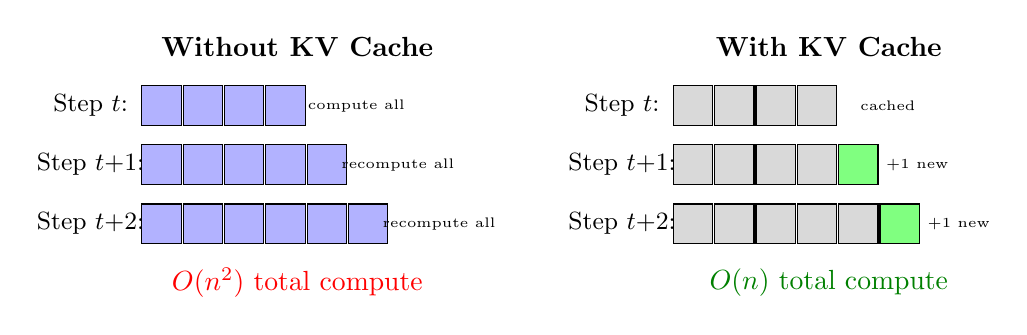
\begin{tikzpicture}[>=stealth, scale=0.75]
        % Without cache
        \begin{scope}
            \node[font=\bfseries] at (3, 4.5) {Without KV Cache};

            % Step t
            \node[font=\small] at (-0.5, 3.5) {Step $t$:};
            \foreach \i in {1,...,4} {
                \node[draw, minimum size=0.5cm, fill=blue!30] at (\i*0.7, 3.5) {};
            }
            \node[font=\tiny] at (4, 3.5) {compute all};

            % Step t+1
            \node[font=\small] at (-0.5, 2.5) {Step $t{+}1$:};
            \foreach \i in {1,...,5} {
                \node[draw, minimum size=0.5cm, fill=blue!30] at (\i*0.7, 2.5) {};
            }
            \node[font=\tiny] at (4.7, 2.5) {recompute all};

            % Step t+2
            \node[font=\small] at (-0.5, 1.5) {Step $t{+}2$:};
            \foreach \i in {1,...,6} {
                \node[draw, minimum size=0.5cm, fill=blue!30] at (\i*0.7, 1.5) {};
            }
            \node[font=\tiny] at (5.4, 1.5) {recompute all};

            \node[red] at (3, 0.5) {$O(n^2)$ total compute};
        \end{scope}

        % With cache
        \begin{scope}[shift={(9, 0)}]
            \node[font=\bfseries] at (3, 4.5) {With KV Cache};

            % Step t
            \node[font=\small] at (-0.5, 3.5) {Step $t$:};
            \foreach \i in {1,...,4} {
                \node[draw, minimum size=0.5cm, fill=gray!30] at (\i*0.7, 3.5) {};
            }
            \node[font=\tiny] at (4, 3.5) {cached};

            % Step t+1
            \node[font=\small] at (-0.5, 2.5) {Step $t{+}1$:};
            \foreach \i in {1,...,4} {
                \node[draw, minimum size=0.5cm, fill=gray!30] at (\i*0.7, 2.5) {};
            }
            \node[draw, minimum size=0.5cm, fill=green!50] at (3.5, 2.5) {};
            \node[font=\tiny] at (4.5, 2.5) {+1 new};

            % Step t+2
            \node[font=\small] at (-0.5, 1.5) {Step $t{+}2$:};
            \foreach \i in {1,...,5} {
                \node[draw, minimum size=0.5cm, fill=gray!30] at (\i*0.7, 1.5) {};
            }
            \node[draw, minimum size=0.5cm, fill=green!50] at (4.2, 1.5) {};
            \node[font=\tiny] at (5.2, 1.5) {+1 new};

            \node[green!50!black] at (3, 0.5) {$O(n)$ total compute};
        \end{scope}
    \end{tikzpicture}
\caption{KV cache avoids recomputation: cached keys/values persist across generation steps.}
\end{figure}

\begin{remark}[KV Cache Memory Cost]
    The cache stores $K, V$ for all layers and all past tokens:
    \[
        \text{Memory} = 2 \times L \times n \times d_{\text{model}} \times \text{bytes per element}
    \]

    For LLaMA-70B with $L = 80$ layers, $d = 8192$, context $n = 4096$, fp16:
    \[
        2 \times 80 \times 4096 \times 8192 \times 2 \text{ bytes} = 10.7 \text{ GB per sequence}
    \]

    This is why long-context models are memory-bound during inference.
\end{remark}

\begin{remark}[Why KV Cache Works with Causal Masking]
    The KV cache relies on causal (autoregressive) attention:
    \begin{itemize}
        \item Past tokens' keys/values don't depend on future tokens
        \item Once computed, $k_i$ and $v_i$ are fixed forever
        \item The query $q_{t+1}$ only needs to attend to $k_1, \ldots, k_{t+1}$
    \end{itemize}

    With bidirectional attention, each new token would change all previous representations, invalidating the cache.
\end{remark}

% ============================================================
\section{Causal Masking}

\begin{definition}[Causal Mask]
    The \textbf{causal mask} (or autoregressive mask) prevents position $i$ from attending to positions $j > i$:
    \[
        M_{ij} = \begin{cases} 0 & \text{if } j \leq i \\ -\infty & \text{if } j > i \end{cases}
    \]
    Applied as: $\text{Attention}(Q, K, V) = \text{softmax}\left(\frac{QK^\top}{\sqrt{d_k}} + M\right) V$
\end{definition}

\begin{figure}[h]
\centering
    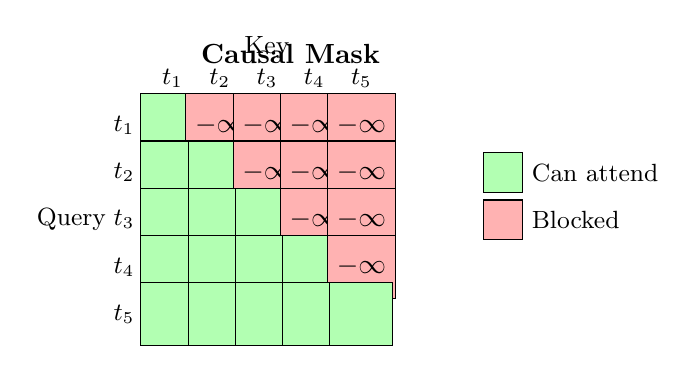
\begin{tikzpicture}[scale=0.6]
        \node[font=\bfseries] at (2.5, 5.5) {Causal Mask};

        % Matrix
        \foreach \i in {0,...,4} {
            \foreach \j in {0,...,4} {
                \pgfmathparse{\j <= \i ? 1 : 0}
                \ifnum\pgfmathresult=1
                    \node[draw, minimum size=0.8cm, fill=green!30] at (\j, 4-\i) {};
                \else
                    \node[draw, minimum size=0.8cm, fill=red!30] at (\j, 4-\i) {$-\infty$};
                \fi
            }
        }

        % Labels
        \node[left] at (-0.6, 4) {\small $t_1$};
        \node[left] at (-0.6, 3) {\small $t_2$};
        \node[left] at (-0.6, 2) {\small $t_3$};
        \node[left] at (-0.6, 1) {\small $t_4$};
        \node[left] at (-0.6, 0) {\small $t_5$};

        \node[above] at (0, 4.6) {\small $t_1$};
        \node[above] at (1, 4.6) {\small $t_2$};
        \node[above] at (2, 4.6) {\small $t_3$};
        \node[above] at (3, 4.6) {\small $t_4$};
        \node[above] at (4, 4.6) {\small $t_5$};

        \node[left, font=\small] at (-1.2, 2) {Query};
        \node[above, font=\small] at (2, 5.2) {Key};

        % Legend
        \node[draw, minimum size=0.5cm, fill=green!30] at (7, 3) {};
        \node[right, font=\small] at (7.4, 3) {Can attend};
        \node[draw, minimum size=0.5cm, fill=red!30] at (7, 2) {};
        \node[right, font=\small] at (7.4, 2) {Blocked};
    \end{tikzpicture}
\caption{Causal mask: lower triangular allows each token to attend only to previous tokens.}
\end{figure}

\begin{remark}[Why Causal Masking is Necessary]
    For autoregressive language modeling:
    \begin{enumerate}
        \item \textbf{Training}: We predict $P(x_t | x_1, \ldots, x_{t-1})$. If token $t$ could see token $t+1$, it would ``cheat''---the task becomes trivial.
        \item \textbf{Inference}: At generation time, future tokens don't exist yet. Training must match this.
        \item \textbf{Parallelism}: Without masking, we'd need sequential training. With masking, we can compute all positions in parallel during training.
    \end{enumerate}
\end{remark}

\begin{remark}[Causal Mask and KV Cache Interaction]
    The causal mask is what makes KV caching possible:
    \begin{itemize}
        \item Token $t$ only attends to tokens $1, \ldots, t$ (causality)
        \item Therefore $k_t$ and $v_t$ only depend on $x_1, \ldots, x_t$
        \item Once computed, these never change regardless of future tokens
        \item Cache is append-only: just add new $k_{t+1}, v_{t+1}$
    \end{itemize}

    Without causality, token $t$'s representation would depend on all tokens, including future ones---caching would be invalid.
\end{remark}

% ============================================================
\section{What Limits Context Window?}

\begin{remark}[Context Window Limitations]
    Several factors limit how long a context a transformer can handle:

    \begin{enumerate}
        \item \textbf{Positional Encodings}: Most are defined for fixed range.
        \begin{itemize}
            \item Learned absolute: $p_1, \ldots, p_N$ are trained embeddings. Position $N+1$ has no embedding.
            \item Sinusoidal: Defined for any position mathematically, but model wasn't trained on long sequences.
            \item RoPE: Rotation angles are defined modulo $2\pi$. With base 10000 and $d=128$, positions beyond $\sim$10000 may have colliding angles.
        \end{itemize}

        \item \textbf{Attention Complexity}: $O(n^2)$ memory and compute. For $n = 1$M tokens, attention matrix has $10^{12}$ entries.

        \item \textbf{Training Distribution}: Model was optimized for sequences of length $\leq N$. Longer sequences are out-of-distribution.

        \item \textbf{Attention Patterns}: Model may learn position-dependent heuristics that break for unseen positions.
    \end{enumerate}
\end{remark}

\begin{remark}[Extending Context Windows]
    Techniques for longer contexts:
    \begin{itemize}
        \item \textbf{Position interpolation}: Scale positions so trained range covers longer sequences. If trained on 4K, scale by $0.5$ to fit 8K into $[0, 4K]$.
        \item \textbf{ALiBi}: Replace positional encodings with linear attention bias based on distance. No position embeddings to extrapolate.
        \item \textbf{Sparse attention}: Only attend to subset of tokens (local window + global tokens). Reduces $O(n^2)$ to $O(n)$.
        \item \textbf{Ring attention}: Distribute attention computation across devices for sequences that don't fit in memory.
    \end{itemize}
\end{remark}

% ============================================================
\section{The Role of Feed-Forward Networks}

\begin{remark}[Why Attention Alone is Insufficient]
    Self-attention has fundamental limitations:
    \begin{enumerate}
        \item \textbf{Linear in values}: Output is a weighted sum of values: $\sum_j \alpha_j v_j$. This is a linear combination---no nonlinearity applied to the content.

        \item \textbf{No position-wise transformation}: Attention mixes information across positions but doesn't transform individual token representations.

        \item \textbf{Rank bottleneck}: With $H$ heads of dimension $d_k$, attention can only produce outputs in a $Hd_k$-dimensional subspace per layer.
    \end{enumerate}
\end{remark}

\begin{remark}[What FFN Provides]
    The feed-forward network $\text{FFN}(x) = W_2 \cdot \text{ReLU}(W_1 x + b_1) + b_2$ contributes:

    \begin{enumerate}
        \item \textbf{Nonlinearity}: ReLU (or GELU/SiLU) introduces nonlinear transformations, enabling the model to learn complex functions.

        \item \textbf{Per-token processing}: Each token is processed independently, allowing position-specific transformations.

        \item \textbf{Capacity expansion}: FFN typically has $d_{\text{ff}} = 4 \times d_{\text{model}}$. This ``expands'' the representation, applies nonlinearity, then ``compresses'' back.

        \item \textbf{Memory/knowledge storage}: Evidence suggests FFN layers store factual associations (``Eiffel Tower $\to$ Paris''). Attention routes information; FFN stores it.
    \end{enumerate}
\end{remark}

\begin{figure}[h]
\centering
    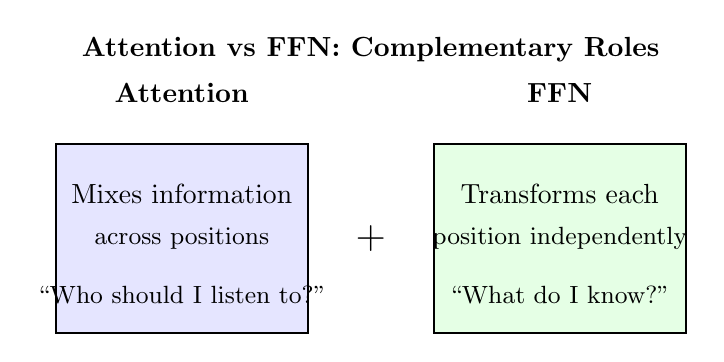
\begin{tikzpicture}[>=stealth, scale=0.8]
        \node[font=\bfseries] at (5, 4.5) {Attention vs FFN: Complementary Roles};

        % Attention
        \begin{scope}
            \node[above] at (2, 3.5) {\textbf{Attention}};
            \draw[thick, fill=blue!10] (0, 0) rectangle (4, 3);
            \node[align=center] at (2, 2.2) {Mixes information};
            \node[align=center] at (2, 1.5) {\small across positions};
            \node[align=center, font=\small] at (2, 0.6) {``Who should I listen to?''};
        \end{scope}

        \node at (5, 1.5) {\Large +};

        % FFN
        \begin{scope}[shift={(6, 0)}]
            \node[above] at (2, 3.5) {\textbf{FFN}};
            \draw[thick, fill=green!10] (0, 0) rectangle (4, 3);
            \node[align=center] at (2, 2.2) {Transforms each};
            \node[align=center] at (2, 1.5) {\small position independently};
            \node[align=center, font=\small] at (2, 0.6) {``What do I know?''};
        \end{scope}
    \end{tikzpicture}
\caption{Attention aggregates across positions; FFN stores and retrieves knowledge at each position.}
\end{figure}

\begin{remark}[Attention is Linear in V]
    Despite softmax nonlinearity in computing weights, attention output is:
    \[
        \text{output}_i = \sum_j \underbrace{\text{softmax}\left(\frac{q_i^\top k_j}{\sqrt{d_k}}\right)}_{\alpha_{ij}} v_j = \sum_j \alpha_{ij} v_j
    \]
    This is a \textbf{weighted average}---a linear combination of the $v_j$. The output lives in the convex hull of values.

    FFN breaks this: $\text{ReLU}(Wx)$ can produce outputs outside any convex hull of inputs.
\end{remark}

% ============================================================
\section{Computational Complexity of Self-Attention}

\begin{theorem}[Self-Attention Complexity]
    For sequence length $n$ and dimension $d$:
    \begin{itemize}
        \item \textbf{Time complexity}: $O(n^2 d)$
        \item \textbf{Memory complexity}: $O(n^2 + nd)$
    \end{itemize}
\end{theorem}

\begin{proof}
    Breaking down the computation:

    \textbf{Computing $Q, K, V$}: Each is $XW$ where $X \in \mathbb{R}^{n \times d}$, $W \in \mathbb{R}^{d \times d_k}$.
    \[
        \text{Cost: } 3 \times O(n \cdot d \cdot d_k) = O(nd^2) \text{ (assuming } d_k \sim d\text{)}
    \]

    \textbf{Computing $QK^\top$}: Matrix multiply $(n \times d_k) \times (d_k \times n) = (n \times n)$.
    \[
        \text{Cost: } O(n^2 d_k) = O(n^2 d)
    \]

    \textbf{Softmax}: Applied to each of $n$ rows of length $n$.
    \[
        \text{Cost: } O(n^2)
    \]

    \textbf{Computing $AV$}: Matrix multiply $(n \times n) \times (n \times d_v) = (n \times d_v)$.
    \[
        \text{Cost: } O(n^2 d_v) = O(n^2 d)
    \]

    \textbf{Total time}: Dominated by $O(n^2 d)$ from $QK^\top$ and $AV$.

    \textbf{Memory}: Must store attention matrix $A \in \mathbb{R}^{n \times n}$ giving $O(n^2)$, plus $Q, K, V, \text{output} \in \mathbb{R}^{n \times d}$ giving $O(nd)$.
\end{proof}

\begin{remark}[Where the Quadratic Term Hurts]
    The $n^2$ term is problematic because:
    \begin{itemize}
        \item \textbf{Memory}: For $n = 100$K, attention matrix is $10^{10}$ floats = 40GB in fp32
        \item \textbf{Compute}: Scales poorly---doubling context 4$\times$ the attention cost
        \item \textbf{Cannot parallelize over sequence}: Must compute all $n^2$ pairs
    \end{itemize}

    Note: The $d$ factor is parallelizable across GPU cores. The $n^2$ factor requires sequential dependency (each query attends to all keys).
\end{remark}

% ============================================================
\section{Permutation Equivariance and Positional Encodings}

\begin{theorem}[Self-Attention is Permutation Equivariant]
    Let $\pi$ be a permutation and $\pi(X)$ the row-permuted input. Then:
    \[
        \text{Attention}(\pi(X)) = \pi(\text{Attention}(X))
    \]
    That is, permuting inputs just permutes outputs the same way.
\end{theorem}

\begin{proof}
    Let $P_\pi$ be the permutation matrix for $\pi$. Then $\pi(X) = P_\pi X$.
    \begin{align*}
        Q' &= P_\pi X W_Q = P_\pi Q \\
        K' &= P_\pi X W_K = P_\pi K \\
        V' &= P_\pi X W_V = P_\pi V
    \end{align*}

    The attention scores:
    \[
        Q'(K')^\top = P_\pi Q (P_\pi K)^\top = P_\pi Q K^\top P_\pi^\top = P_\pi A P_\pi^\top
    \]

    After softmax (applied row-wise, preserving structure):
    \[
        A' = P_\pi A P_\pi^\top
    \]

    The output:
    \[
        A' V' = P_\pi A P_\pi^\top P_\pi V = P_\pi A V = P_\pi \cdot \text{Attention}(X)
    \]
\end{proof}

\begin{remark}[Consequence: Attention Sees a Set, Not a Sequence]
    Without positional encodings:
    \begin{itemize}
        \item ``The cat sat on the mat'' $\equiv$ ``mat the on sat cat The'' (same bag of tokens)
        \item Word order carries no information
        \item Language structure is lost
    \end{itemize}

    \textbf{Positional encodings break this symmetry} by making $x_i \neq x_j$ even if tokens are identical, because $x_i + p_i \neq x_j + p_j$.
\end{remark}

\begin{figure}[h]
\centering
    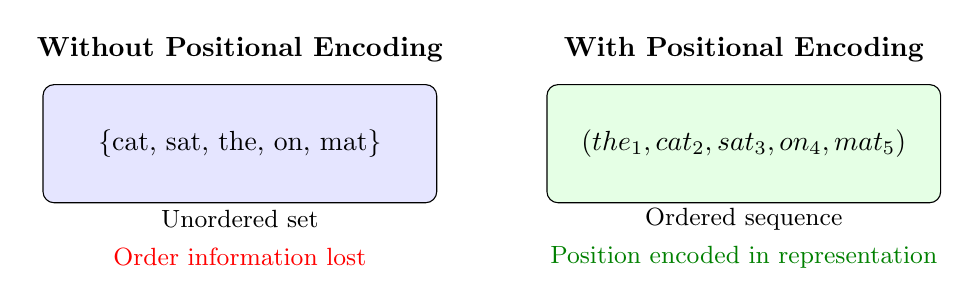
\begin{tikzpicture}[>=stealth, scale=0.8]
        % Without PE
        \begin{scope}
            \node[font=\bfseries] at (2.5, 3.5) {Without Positional Encoding};
            \node[draw, rounded corners, fill=blue!10, minimum width=5cm, minimum height=1.5cm] at (2.5, 2) {};
            \node at (2.5, 2) {$\{$cat, sat, the, on, mat$\}$};
            \node[font=\small] at (2.5, 0.8) {Unordered set};
            \node[font=\small, red] at (2.5, 0.2) {Order information lost};
        \end{scope}

        % With PE
        \begin{scope}[shift={(8, 0)}]
            \node[font=\bfseries] at (2.5, 3.5) {With Positional Encoding};
            \node[draw, rounded corners, fill=green!10, minimum width=5cm, minimum height=1.5cm] at (2.5, 2) {};
            \node at (2.5, 2) {$(the_1, cat_2, sat_3, on_4, mat_5)$};
            \node[font=\small] at (2.5, 0.8) {Ordered sequence};
            \node[font=\small, green!50!black] at (2.5, 0.2) {Position encoded in representation};
        \end{scope}
    \end{tikzpicture}
\caption{Positional encodings break permutation symmetry, converting sets into ordered sequences.}
\end{figure}

% ============================================================
\section{Why Transformers Excel at Lexical Matching}

\begin{remark}[Attention as Exact Match]
    Self-attention computes $q_i^\top k_j$---a dot product measuring similarity. For identical tokens:
    \[
        q_i = W_Q x_i, \quad k_j = W_K x_j
    \]
    If $x_i = x_j$ (same token), then $q_i^\top k_j$ is maximized when $W_Q, W_K$ are learned to detect this.

    The model can easily learn: ``attend strongly to tokens that match exactly.''
\end{remark}

\begin{remark}[Induction Heads Enable String Matching]
    Recall induction heads: $[A][B] \cdots [A] \to [B]$

    This is precisely lexical/string matching:
    \begin{enumerate}
        \item Find previous occurrence of current token (lexical match)
        \item Copy what came next (pattern completion)
    \end{enumerate}

    This emerges naturally from the attention mechanism---no explicit string matching algorithm needed.
\end{remark}

\begin{remark}[Why Lexical Match is Easy for Attention]
    Consider the attention score for matching tokens $x_i = x_j$:
    \[
        \text{score}_{ij} = (W_Q x_i)^\top (W_K x_j) = x_i^\top W_Q^\top W_K x_j
    \]

    If $W_Q^\top W_K \approx I$ (identity), then $\text{score}_{ij} \approx x_i^\top x_j$, which is maximized when $x_i = x_j$.

    Learning $W_Q^\top W_K \approx I$ is trivial---just initialize appropriately. This is why transformers are ``born'' with some string-matching ability.
\end{remark}

% ============================================================
\section{Depth vs Width in Transformers}

\begin{remark}[Why Depth Helps Compositional Reasoning]
    Each transformer layer can be seen as one ``step'' of computation:
    \begin{itemize}
        \item Layer 1: Direct token relationships (adjacent words, simple patterns)
        \item Layer 2: Compositions of layer 1 patterns (phrases, local syntax)
        \item Layer $k$: $k$-step reasoning chains
    \end{itemize}

    For tasks requiring $k$ sequential reasoning steps, you need at least $k$ layers. \textbf{Depth enables sequential composition.}
\end{remark}

\begin{remark}[Why Width (More Heads) is Different]
    Adding more attention heads within a layer:
    \begin{itemize}
        \item Heads operate \textbf{in parallel}, not sequentially
        \item Each head captures a \textbf{different} relationship type
        \item More heads = more relationship types per layer, but not deeper reasoning
    \end{itemize}

    Analogy:
    \begin{itemize}
        \item \textbf{Depth}: More steps in a proof (sequential)
        \item \textbf{Width}: More facts available at each step (parallel)
    \end{itemize}

    You can't replace sequential reasoning with more parallel processing---some computations are inherently serial.
\end{remark}

\begin{figure}[h]
\centering
    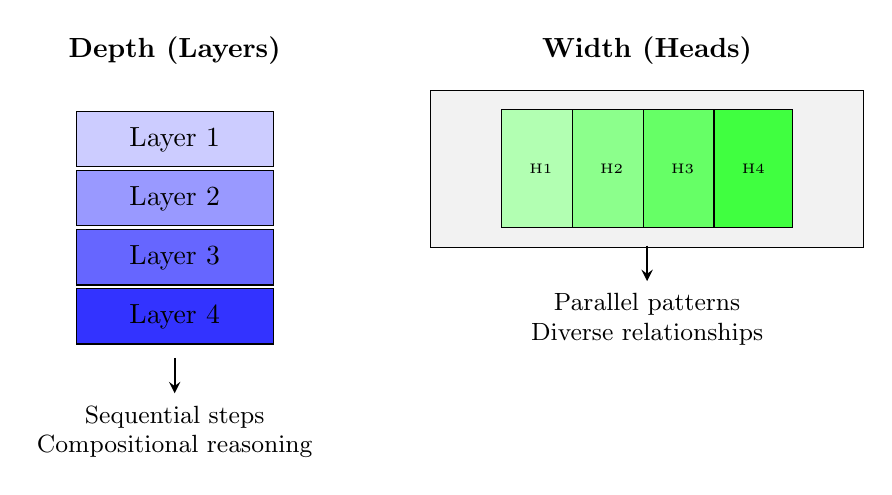
\begin{tikzpicture}[>=stealth, scale=0.75]
        % Depth
        \begin{scope}
            \node[font=\bfseries] at (1.5, 5) {Depth (Layers)};
            \foreach \i in {0,...,3} {
                \node[draw, minimum width=2.5cm, minimum height=0.7cm, fill=blue!\the\numexpr 20+\i*20\relax] at (1.5, 3.5 - \i*1) {Layer \the\numexpr\i+1\relax};
            }
            \draw[->, thick] (1.5, -0.2) -- (1.5, -0.8);
            \node[font=\small] at (1.5, -1.2) {Sequential steps};
            \node[font=\small] at (1.5, -1.7) {Compositional reasoning};
        \end{scope}

        % Width
        \begin{scope}[shift={(7, 0)}]
            \node[font=\bfseries] at (2.5, 5) {Width (Heads)};
            \node[draw, minimum width=5.5cm, minimum height=2cm, fill=gray!10] at (2.5, 3) {};
            \foreach \i in {0,...,3} {
                \node[draw, minimum width=1cm, minimum height=1.5cm, fill=green!\the\numexpr 30+\i*15\relax] at (0.7 + \i*1.2, 3) {\tiny H\the\numexpr\i+1\relax};
            }
            \draw[->, thick] (2.5, 1.7) -- (2.5, 1.1);
            \node[font=\small] at (2.5, 0.7) {Parallel patterns};
            \node[font=\small] at (2.5, 0.2) {Diverse relationships};
        \end{scope}
    \end{tikzpicture}
\caption{Depth vs width in transformer architecture: depth enables sequential compositional reasoning while width enables parallel pattern matching.}
\end{figure}
